%% using aastex version 6.31
\documentclass[twocolumn]{aastex631}
\usepackage{CJK}
% \usepackage{lineno}
% \linenumbers

\newcommand{\sn}{SN\,2022joj}
\newcommand{\trmax}{$t_{r_\mathrm{ZTF},\mathrm{max}}$}
\newcommand{\tfl}{$t_\mathrm{fl}$}
\newcommand{\Mch}{$M_\mathrm{Ch}$}
\newcommand{\kms}{$\mathrm{km}\,\mathrm{s}^{-1}$}
\newcommand{\Ni}{$^{56}\mathrm{Ni}$}
\newcommand{\Msun}{\mathrm{M_\odot}}
\newcommand{\adam}[1]{\textcolor{orange}{[AAM: #1]}}
\newcommand{\chang}[1]{\textcolor{blue}{[Chang: #1]}}

\shorttitle{\sn}
\shortauthors{Liu et al.}
\graphicspath{{./}{figures/}}


\begin{document}
\begin{CJK*}{UTF8}{gbsn}

\title{SN\,2022joj}

%main contributors
\author[0000-0002-7866-4531]{Chang~Liu}
\affil{Department of Physics and Astronomy, Northwestern University, 2145 Sheridan Rd, Evanston, IL 60208, USA}
\affil{Center for Interdisciplinary Exploration and Research in Astrophysics (CIERA), Northwestern University, 1800 Sherman Ave, Evanston, IL 60201, USA}

\author[0000-0001-9515-478X]{Adam~A.~Miller}
\affil{Department of Physics and Astronomy, Northwestern University, 2145 Sheridan Rd, Evanston, IL 60208, USA}
\affil{Center for Interdisciplinary Exploration and Research in Astrophysics (CIERA), Northwestern University, 1800 Sherman Ave, Evanston, IL 60201, USA}

\author{Fantastic Astronomers}
\begin{abstract} 
%

%
\end{abstract}

\keywords{Supernovae (1668), Type Ia supernovae (1728), White dwarf stars (1799), Observational astronomy (1145), Surveys (1671)}

\section{Introduction} \label{sec:intro}

\chang{For the introduction I don't think we need the full history of peculiar SNe\,Ia. I think we can note that there is compelling evidence for multiple progenitor channels, and then highlight Double Detonations, and then point out that some features are consistent across simulations -- e.g., very massive He shells produce very red transients -- while other features depend on 1D, 2D, LTE/non-LTE, etc. Then you can say we present new observations of a peculiar SN\,Ia that initially showed red colors but eventually evolved to the red.}

\section{Observations} \label{sec:obs}
\subsection{Discovery \& Classification}
\sn\ was discovered by the Zwicky Transient Facility \citep[ZTF;][]{Bellm_ZTF_2019a,Graham_ZTF_2019,Dekany_ZTF_2020} on 2022 May 08.298 (UT dates are used throughout the paper; MJD 59707.298) with the 48\,inch Samuel Oschin Telescope (P48) at Palomar Observatory. It was detected with $r_\mathrm{ZTF}=19.13\pm0.06$\,mag at $\alpha_\mathrm{J2000}=14^\mathrm{h}41^\mathrm{m}40\fs08$, $\delta_\mathrm{J2000}=+03\degr00'24\farcs{14}$ and announced to the public by \citet{Fremling_2022TNSTR}. \sn\ was detected via the ZOGY image differencing algorithm \citep{Zackay_imagesub_2016}, which is utilized by the automated ZTF discovery pipeline \citep{Masci_ZTF_2019}. A real-time alert \citep{Patterson_ZTFalert_2019} was generated as the candidate passed internal machine-learning thresholds \citep[e.g.,][]{Duev_ZTFML_2019,Mahabal_ZTFML_2019}, and the internal designation ZTF22aajijjf was assigned. The last 3-$\sigma$ nondetection limits the brightness to $r_\mathrm{ZTF}>21.48$\,mag on 2022 May 03.27 (MJD 59702.27; 5.03\,days before the first detection -- \chang{Is this limit from forced photometry or from the alert packets, either way we should make this clear, and if it's alert packet info we should highlight that the forced photometry provides better limits later on}). \chang{I think we've done this, but have we investigated ATLAS photometry - in particular limits on the time of explosion - at all?}

The first spectrum was obtained on 2022 May 11.288 by \citet{Newsome_2022TNSCR}, who found a best fit to a young Type I SN at $z=0.03$ using the \texttt{Supernova Identification (SNID)} algorithm \citep{Blondin_SNID_2007}. In this early spectrum, prominent \ion{Si}{2} $\lambda$6355 and \ion{Ca}{2} infrared triplet (IRT) absorption suggest a SN\,Ia classification, but the overall spectral shape, featuring a relatively red continuum (see Figure~\ref{fig:spec_seq}), is atypical for a normal SN\,Ia at this phase. \citet{Chu_2022TNSCR} use a maximum luminosity spectrum to indisputably classify \sn\ as a SN\,Ia based on its blue color and persistent \ion{Si}{2} features.

\subsection{Host Galaxy}
The host of \sn\ is a dwarf galaxy at $\alpha_\mathrm{J2000}=14^\mathrm{h}41^\mathrm{m}40\fs04$, $\delta_\mathrm{J2000}=+03\degr00'24\farcs{53}$, cataloged in the DESI Legacy Survey \citep[LS;][]{Dey_LS_2019}. \sn\ has a projected offset of only $0\farcs{5}$ to the host \chang{Do we have an uncertainty on this?}. On 2023 April 26, we took a spectrum of both the SN and the host using the Low Resolution Imaging Spectrometer \citep[LRIS;][]{Keck_1995} on the Keck I 10m telescope \chang{pretty sure the ref if LRIS not all Keck}. We placed the slit across both the center of the galaxy and the position of the SN (Figure~\ref{fig:host_spec}), with a total integration time of 3600\,s \chang{mention that we use the ADC?}. The spectrum was reduced with the \texttt{PypeIt} package \citep{pypeit:joss_pub}. While the continuum spectrum of the host was still outshined by the SN, we detected a potential host emission line at 6742.4\,\r{A} with a signal-to-noise ratio (S/N) of $\sim$5 \chang{probably worth a precise estimate of the SNR}. If this is associated with the H$\alpha$ emission, the corresponding redshift of the host galaxy is $z=0.02736$, which is in general agreement with the estimated value $z=0.03$ by matching the SN spectra to \texttt{SNID} templates \citep{Newsome_2022TNSCR}. In the 2D spectrum (Figure~\ref{fig:host_spec}), the trace is dominated by the light of the SN in the nebular phase, while the center of this emission feature has a offset of $\sim$3--4 pixels to the center of the trace. The CCDs equipped on LRIS have a pixel scale of $0\farcs135$/pixel, so this offset corresponds to an angular offset of $\sim$$0\farcs4$--$0\farcs5$, consistent with the archival value. This indicates that the H$\alpha$ detection is real.

\chang{No mention of the Binospec spectrum? Did you ever check the Harvard reduction vs. pypeit? Does either reduction show evidence for Halpha at the correct redshift?}

We estimate the distance modulus of \sn\ in the following way. We first use the 2M++ model \citep{Carrick2015_2M++} to estimate the peculiar velocity of the host galaxy to be $383\pm250$\,\kms. Then the peculiar velocity is combined with the recession velocity in the frame of the cosmic microwave background (CMB) $v_\mathrm{CMB}=8424$\,\kms, which yields a net Hubble recession rate of $8193\pm250$\,\kms. Using cosmological parameters $H_0 = 70\,\mathrm{km\,s^{-1}\,Mpc^{-1}}$, $\Omega_M=0.3$, and $\Omega_\Lambda=0.7$, the estimated luminosity distance to \sn\ is 119.5\,Mpc, equivalent to a distance modulus of $35.39\pm0.03$\,mag.

\subsection{Optical Photometry}
\sn\ was monitored in $g_\mathrm{ZTF}$, $r_\mathrm{ZTF}$, and $i_\mathrm{ZTF}$ by ZTF as part of its ongoing Northern Sky Survey \citep{Bellm_ZTF_2019b}. The $i_\mathrm{ZTF}$ data only cover the decline from the peak. We adopt a Galactic extinction of $E(B-V)_\mathrm{MW}=0.032$\,mag \chang{E(B-V) shouldn't be broken over the end of the line - I think AAS provides a macro for E(B-V)} \citep{Schlafly2011}, and correct all photometry using the extinction model from \citet{Fitzpatrick1999} assuming $R_V=3.1$. We do not find any \ion{Na}{1} D absorption at the redshift of the host galaxy, indicating that the extinction from the host is negligible. The blue $g_\mathrm{ZTF}-r_\mathrm{ZTF}$ color ($\sim$$-0.2$\,mag) near maximum luminosity after correcting for the Galactic extinction is also consistent with no additional reddening from the host. Therefore we assume $E(B-V)_\mathrm{host}=0$.

The basic photometric properties of \sn\ are listed in Table~\ref{tab:basics}. We do not include the maximum $i_\mathrm{ZTF}$-band properties, which are relatively uncertain due to the low cadance in $i_\mathrm{ZTF}$ around peak. 
The forced-photometry light curves\footnote{\url{https://web.ipac.caltech.edu/staff/fmasci/ztf/forcedphot.pdf}} in $g_\mathrm{ZTF}$ and $r_\mathrm{ZTF}$ (in absolute magnitudes) are shown in Figure~\ref{fig:lc}. These light curves are reduced using the pipeline from A. A. Miller et al. (2023, in preparation); see also \citet{Yao_2019}. \chang{Frank has posted a paper on the arXiv, or is about to, so we should cite that directly. The first step in the process is the \texttt{Forced Photometry Service} from ZTF}

\begin{deluxetable*}{lcccccc} \label{tab:basics}
\tabletypesize{\scriptsize}
\tablewidth{0pt}
\tablecaption{Basic photometric properties of \sn.}
\tablehead{
\multicolumn{7}{c}{Rise (flux $\le$$40\%$ of peak luminosity)}
}
\startdata
$t_\mathrm{fl}$ (MJD) & \multicolumn{6}{c}{$59703.16^{+0.70}_{-0.58}$} \\
$\alpha_{\mathrm{ZTF}, r}$ & \multicolumn{6}{c}{$2.18^{+0.20}_{-0.24}$} \\
$\alpha_{\mathrm{ATLAS}, o}$ & \multicolumn{6}{c}{$2.37^{+0.48}_{-0.20}$} \\
$t_{\mathrm{fl}, \alpha=2}$ (MJD) & \multicolumn{6}{c}{$59703.66 ^{+0.10}_{-0.11}$} \\
\hline
\multicolumn{7}{c}{Maximum luminosity}\\[+0.1cm]
\hline
Filters & $g_\mathrm{ZTF}$ & $r_\mathrm{ZTF}$ & $B$ & $V$ & $R$ & $I$\\
$t_\mathrm{max,poly}$ (MJD) & $59722.66\pm0.21$ & $59725.54\pm0.09$ & $59722.77\pm0.30$ & $59724.88\pm0.28$ & $59724.61\pm0.28$ & $59720.73\pm0.27$\\
$M_\mathrm{max,poly}$ (mag) & $-19.693\pm0.014$ & $-19.492\pm0.004$ & $-19.456\pm0.011$ & $-19.544\pm0.009$ & $-19.496\pm0.009$ & $-19.222\pm0.011$\\
%$t_\mathrm{max,SALT}$ (MJD) & $59724.16\pm0.04$ & $59725.26\pm0.03$ & $59723.36\pm0.04$\\
%$M_\mathrm{max,SALT}$ (mag) & $-19.663\pm0.007$ & $-19.409\pm0.002$ & $-19.780\pm0.009$\\
\enddata
\tablecomments{Parameters are defined in the text. The absolute magnitudes have been corrected for Galactic extinction. The uncertainty in the distance modulus (0.03\,mag) and the systematics in the polynomial models are not included.}
\end{deluxetable*}


\begin{figure*}
    \centering
    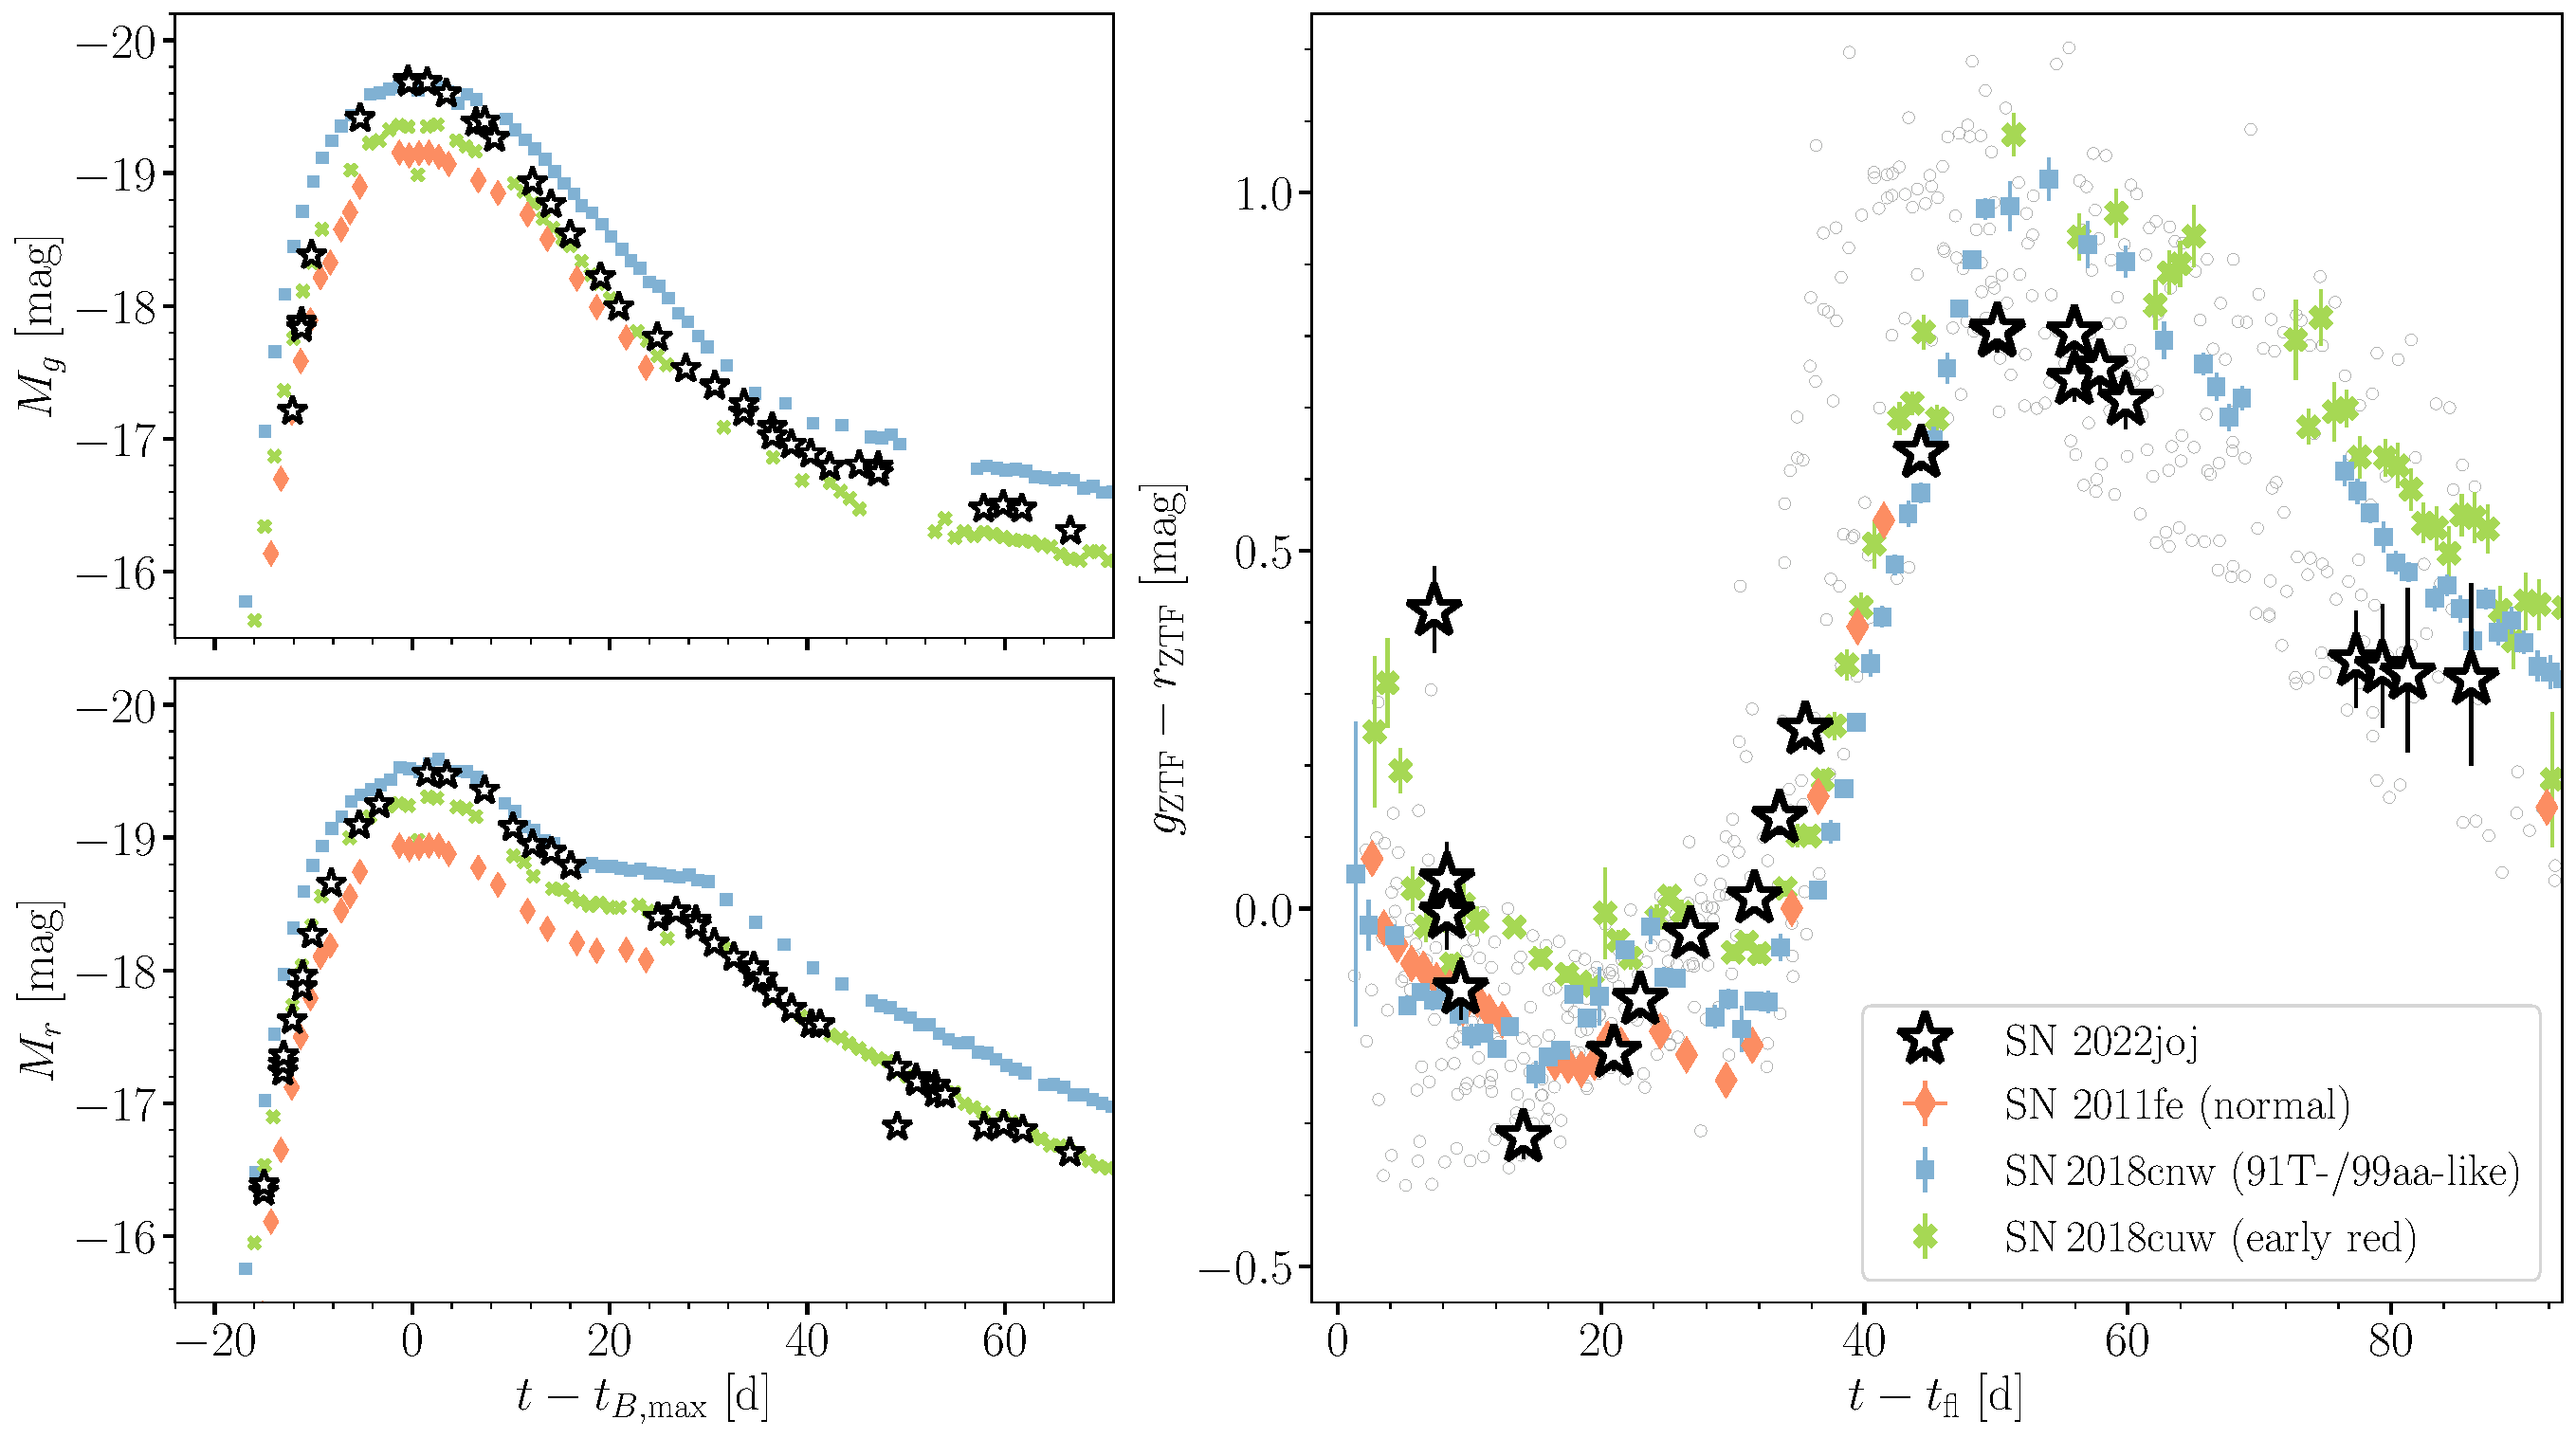
\includegraphics[width=\textwidth]{photometry.pdf}
    \label{fig:lc}
    \caption{Comparison of the photometric properties of \sn\ with SN\,2011fe \citep[normal Ia;][]{Pereira_2013}, SN\,2018cnw (91T-/99aa-like), and SN\,2018cuw (normal Ia with a red early color). \textit{Left}: multiband light curves. The upper (lower) panel shows the evolution in the $g$-band ($r$-band) absolute magnitude. %{The arrows mark the 5$\sigma$ limit of the last nondetections of \sn\ in $g_\mathrm{ZTF}$ and $r_\mathrm{ZTF}$.} 
    \textit{Right}: $g_\mathrm{ZTF}-r_\mathrm{ZTF}$ color evolution. %For each object, the peak epoch is marked by a vertical line with the corresponding color on the bottom axis. 
    The gray circles denote the color evolution of 14 nearby ($z\le0.05$) SNe\,Ia (open circles) from the ZTF sample with prompt observations within 5\,days of first light \citep{Bulla2020}. Note that $K$-corrections have not been applied.}
\end{figure*}

\subsection{Optical Spectroscopy}\label{sec:optical_spec}

We obtained a series of optical spectra of \sn\ using the Spectral Energy Distribution Machine \citep[SEDM;][]{SEDM_2018} on the automated 60\,inch telescope \citep[P60;][]{P60_2006} at Palomar observatory, the Andalucia Faint Object Spectrograph and Camera (ALFOSC)\footnote{\url{http://www.not.iac.es/instruments/alfosc/}} installed at the Nordic Optical Telescope (NOT), the SPectrograph for the Rapid Acquisition of Transients \citep[SPRAT;][]{SPRAT_2014} on the 2\,m Liverpool Telescope \citep[LT;][]{LT_2004}, FLOYDS spectrograph\footnote{\url{https://lco.global/observatory/instruments/floyds/}} on the 2m Faulkes Telescope South (FTS) at Siding Spring as part of the Las Cumbres Observatory global telescope (LCOGT) network \citep{LCOGT_2013}, Binospec \citep{Binospec_2019} on the 6.5m MMT telescope, and LRIS on the Keck I 10m telescope \chang{already cited LRIS}. With the exception of observations obtained with SEDM, all spectra were reduced using standard procedures \citep[e.g.,][]{Matheson_2000}. The SEDM spectra were reduced using the custom \texttt{pysedm} software package \citep{Rigault_pysedm_2019}. Details of the spectroscopic observations are listed in Table~\ref{tab:spec}. The resulting spectral sequence is shown in Figure~\ref{fig:spec_seq}. All the spectra listed in Table 1 will be available on WISeREP \citep{wiserep_2012}.

We also include the spectrum uploaded to the Transient Name Server (TNS) by \citet{Newsome_2022TNSCR} in our analysis, which was obtained using the FLOYDS spectrograph on the 2m Faulkes Telescope North (FTN) at Haleakala.

\begin{figure}
    \centering
    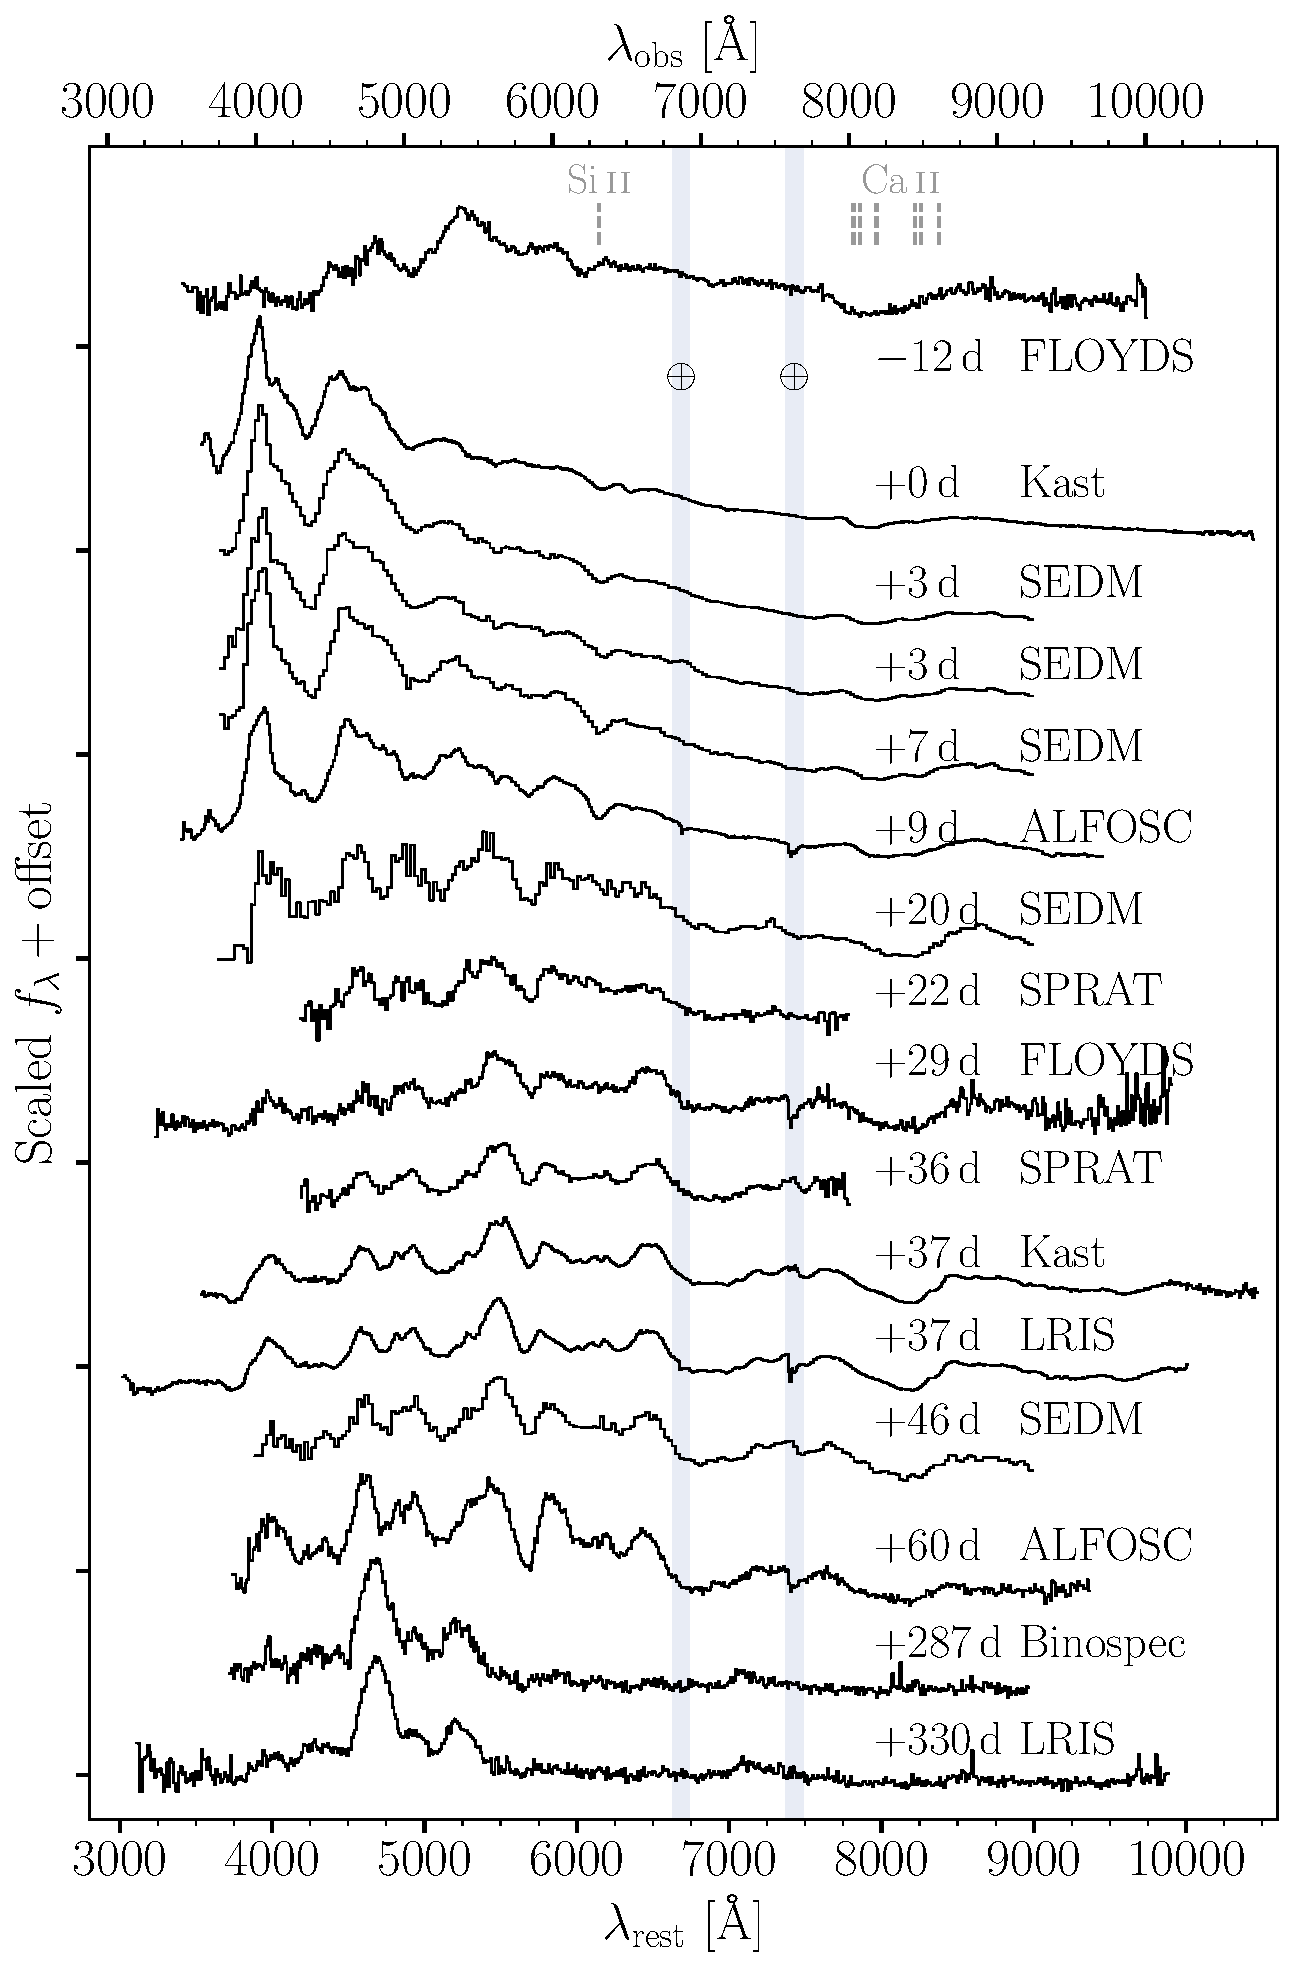
\includegraphics[width=\linewidth]{SN2022joj_spectral_sequence.pdf}
    \caption{Optical spectral sequence of \sn\ \chang{reminder that the caption can be used to tell the story - for instance you could highlight the red to blue transition which is plainly evident at the top of this figure}. Rest-frame phase relative to the $B$-band peak and the instrument used are listed next to each spectrum. Spectra have been corrected for $E(B-V)_\mathrm{MW} = 0.032$\,mag and are shown in gray. The black lines are binned spectra with a bin size of 10\,\AA, except for the SEDM spectra, whose resolution is lower than the bin size. The corresponding wavelengths of the \ion{Si}{2} $\lambda$6355 line (with an expansion velocity of 10,000\,\kms) and the \ion{Ca}{2} IRT (with expansion velocities of both 10,000\,\kms and 25,000\,\kms) are marked by the vertical dashed lines. The strong optical telluric features are marked by the blue shaded region. \chang{mention that this is A and B band?}}
    \label{fig:spec_seq}
\end{figure}

\begin{deluxetable}{lrccc} \label{tab:spec}
\tabletypesize{\scriptsize}
\tablewidth{0pt}
\tablecaption{Spectroscopic observations of \sn\label{tab:spectra}.}
\tablehead{
\colhead{$t_\mathrm{obs}$} &
\colhead{Phase} &
\colhead{Telescope/} &
\colhead{$R$} &
\colhead{Range} \\
\colhead{(MJD)} &
\colhead{(days)} &
\colhead{Instrument} &
\colhead{$(\lambda/\Delta\lambda)$} &
\colhead{(\AA)}
}
\startdata
%59,710.29 &  $-$12.5 & LCO/FLOYDS-N & 400--700 & 3500--10000\\% & --\\
59,710.29 &  $-$12.1 & FTN/FLOYDS-N & 550 & 3500--10000\\% & --\\
59,725.34 &  $+$2.5  & P60/SEDM & 100 & 3770--9220 \\%&  1.33\\
59,725.43 &  $+$2.6  & P60/SEDM & 100 & 3770--9220 \\%&  2.29\\
59,732.02 &  $+$9.0  & NOT/ALFOSC & 360 & 3500--9700 \\%& 1.17\\
59,744.96 & $+$21.6  & LT/SPRAT & 350 & 4020--7990 \\%& 1.28\\ % 300/7500, 4.60 A/pix, FWHM ~ 10 A
59,752.50 & $+$29.0  & FTS/FLOYDS-S & 550 & 3500--10000 \\%& 1.28\\
59,759.92 & $+$36.2  & LT/SPRAT & 350 & 4020--7990 \\%&1.07\\
59,760.37 & $+$36.6  & Keck I/LRIS & 1100 & 3100--10280 \\%&  1.27\\
59,784.89 & $+$60.5  & NOT/ALFOSC & 360 & 3850--9620 \\%& 2.04\\
60,017.42 & $+$286.8 & MMT/Binospec & 1340 & 3830--9210 \\%& 1.31\\
60,061.56 & $+$329.8 & Keck I/LRIS & 1100 & 3200--10150 \\%& 2.16\\
\enddata
\tablecomments{Phase is measured relative to the $B$-band peak in the rest frame of the host galaxy. The resolution $R$ is reported for the central region of the spectrum.}
\end{deluxetable}


\begin{figure*}
    \centering
    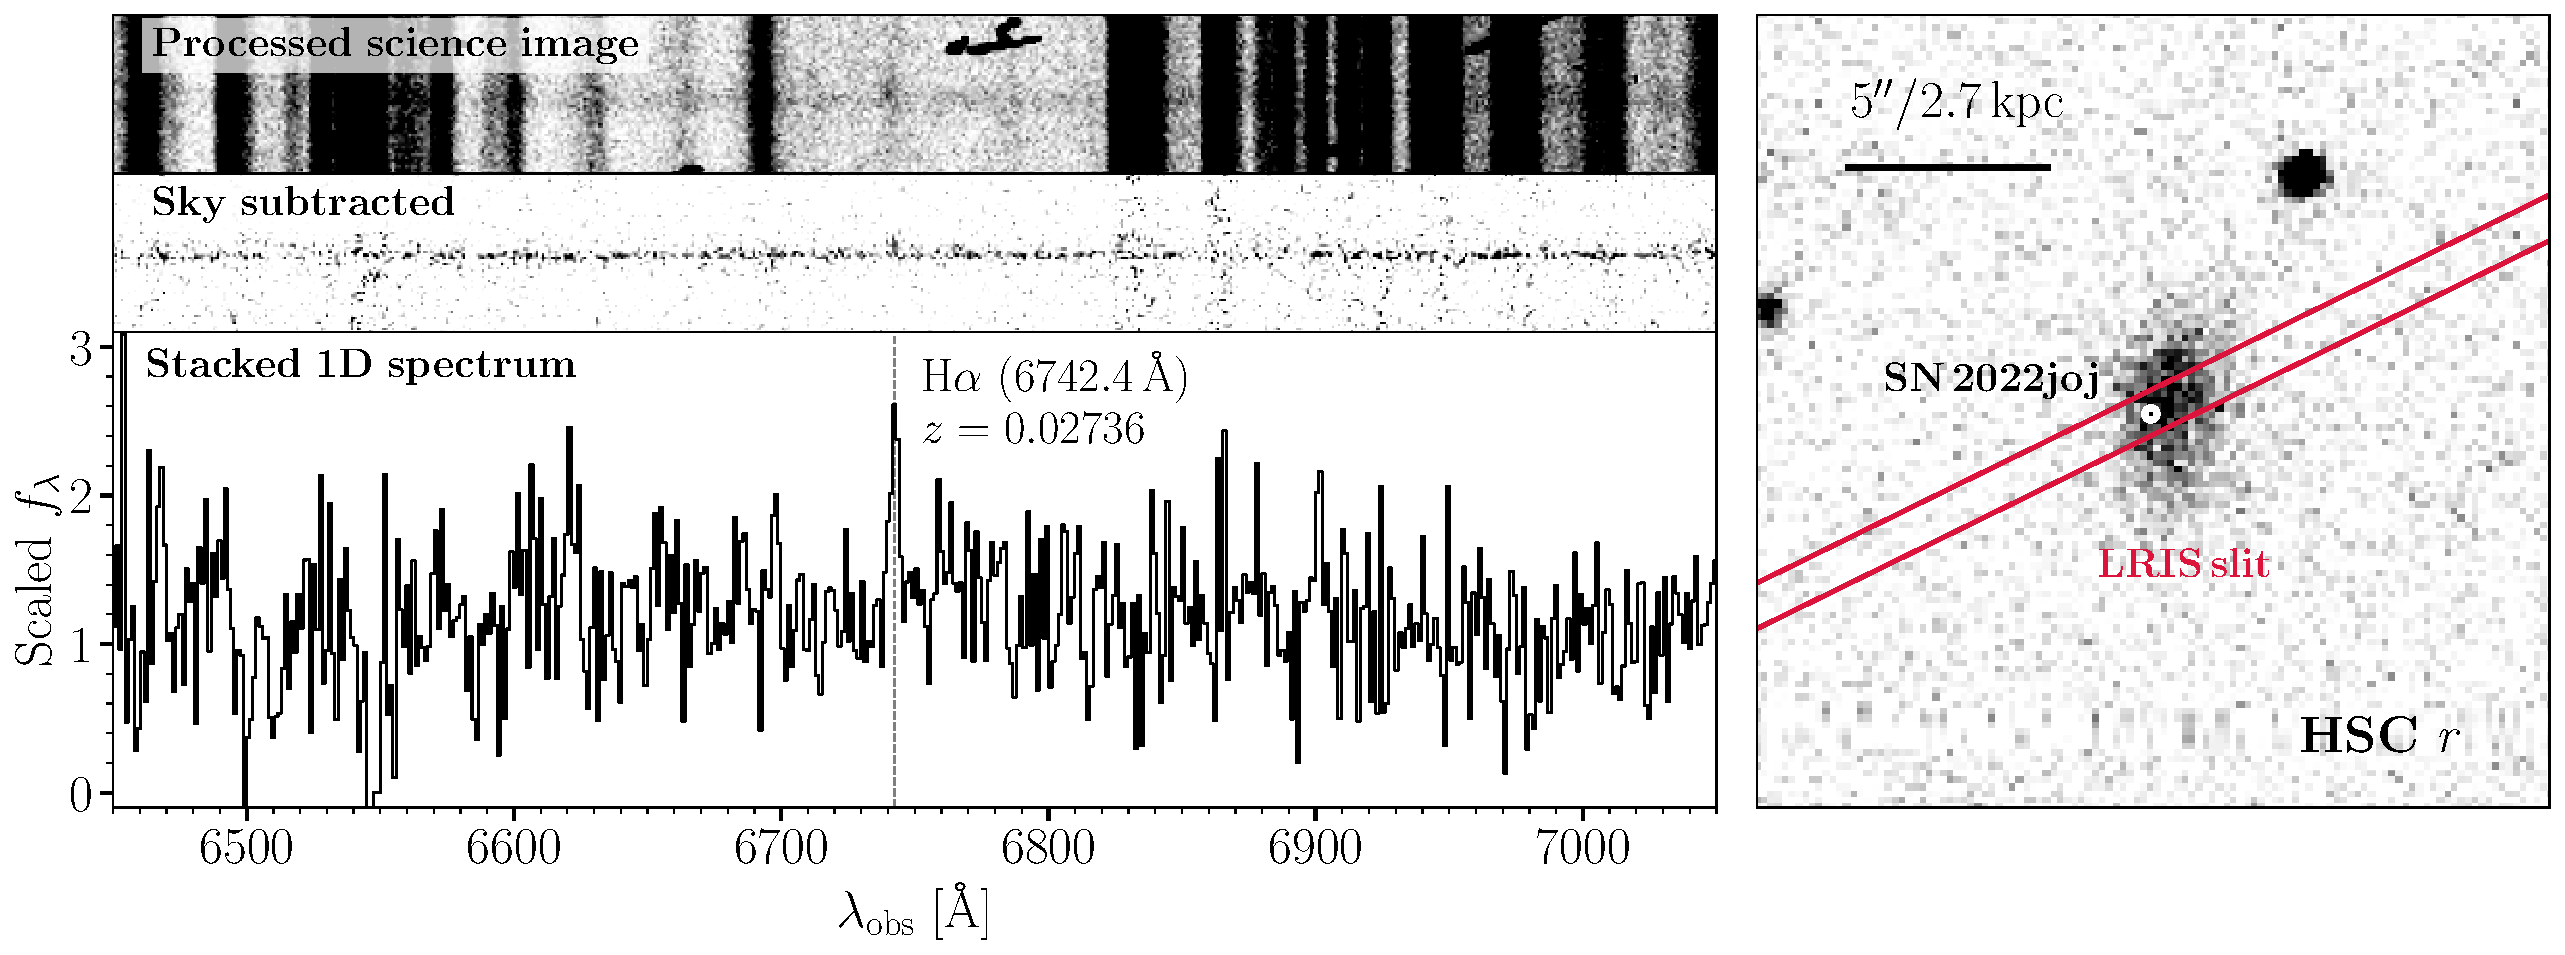
\includegraphics[width=\linewidth]{host_spec.pdf}
    \caption{The LRIS spectrum reveals an H$\alpha$ emission line from the host galaxy at 6742.4\,\AA, corresponding to a redshift $z=0.02736$. \textit{Left:} the H$\alpha$ emission in the observed 2D and 1D spectrum. %\textit{Top left:} the calibrated science image with the trace of the SN/host. \textit{Center left:} the trace with the sky background subtracted. \textit{Bottom left:} the corresponding 1D spectrum.
    \textit{Right:} image of \sn\ and its host galaxy with the orientation of the LRIS slit overplotted.    
    }
    \label{fig:host_spec}
\end{figure*}

\section{Analysis} \label{sec:analysis}
\subsection{Early Light Curves and the First Light}
To estimate the time of first light ($t_\mathrm{fl}$), we assume an initial power-law rise in the broad-band flux $f(t)$,
$$
f(t) = A (t-t_\mathrm{fl})^\alpha,
$$
where $A$ is a constant and $\alpha$ is the power-law index \chang{do you only include flux up to 40\% of peak luminosity - if so this is an important detail, and a reasonable place to cite my 2020 paper}. We only fit the $r_\mathrm{ZTF}$-band forced-photometry light curve to the power-law model as the coverage is significantly worse in the $g_\mathrm{ZTF}$ and $i_\mathrm{ZTF}$ bands at this phase (see Section~\ref{sec:analysis_phot}). We estimate $\alpha$, $t_\mathrm{fl}$, and $\ln A$ in a Bayesian approach by sampling their posterior distributions with Markov Chain Monte Carlo (MCMC) using the package \texttt{PyMC} \citep{pymc_2016} \chang{we should mention the priors somewhere}. We find that the $r_\mathrm{ZTF}$-band light curve is consistent with a power-law rise with $\alpha=2.32^{+0.23}_{-0.29}$, in which the first detection in $r_\mathrm{ZTF}$ is $4.55^{+0.86}_{-0.67}$\,days after the first light. This estimate is consistent with the $\alpha=2$ fireball model. When fixing $\alpha=2$, the model still fits the light curve well, but the estimated $t_\mathrm{fl}$ is $\sim$1\,day later (see Table~\ref{tab:basics}). We do not find any correlated residuals as evidence for a flux excess in $r_\mathrm{ZTF}$ after $\sim$5\,days since $t_\mathrm{fl}$, although a flux excess before the first detection could not be ruled out.


\subsection{Photometric Properties} \label{sec:analysis_phot}
\sn\ shows a few peculiar photometric features compared to normal SNe\,Ia. In Figure~\ref{fig:lc}, we compare the $g_\mathrm{ZTF}$ and $r_\mathrm{ZTF}$ light curves and the $g_\mathrm{ZTF} - r_\mathrm{ZTF}$ color evolution of \sn\ with those of the well-observed normal SN\,Ia, SN\,2011fe,\footnote{We show the synthetic photometry in $g_\mathrm{ZTF}$ and $r_\mathrm{ZTF}$ calculated using the spectrophotometric sequence from \citet{Pereira_2013}.} as well as SN\,2018cnw (ZTF18abauprj) and SN\,2018cuw (ZTF18abcflnz) from a sample of SNe\,Ia with prompt observations within 5\,days of first light by ZTF \citep{Yao_2019,Bulla2020}. 
SN\,2018cnw is slightly overluminous at peak, and belongs to either the SN\,1999aa-like \citep[99aa-like;][]{Garavini_99aa_2004} or SN\,1991T-like \citep[91T-like;][]{Filippenko_91T_1992} subclass of SNe\,Ia, while SN\,2018cuw is a normal SN\,Ia with a red $g_\mathrm{ZTF} - r_\mathrm{ZTF}$ color comparable to that of \sn\ $\sim$15\,d prior to peak. 

Around maximum brightness, \sn\ is overluminous, comparable to SN\,2018cnw, and $\sim$0.5\,mag brighter than SN\,2011fe in both $g_\mathrm{ZTF}$ and $r_\mathrm{ZTF}$. But \sn\ clearly stands out due to its fast evolution in $g_\mathrm{ZTF}$. While \sn\ and SN\,2018cnw show a similar maximum brightness in $g_\mathrm{ZTF}$, upon the earliest detection in $g_\mathrm{ZTF}$ at $\sim$$-13$\,days \chang{this clause is confusing ebcause it isn't clear if this is first detection of joj or cnw}, the corresponding absolute magnitude ($-17.2$\,mag) is $\sim$0.8\,mag fainter than that of SN\,2018cnw at a similar phase. This means on average, \sn\ rises faster than SN\,2018cnw by $\sim$$0.06\,\mathrm{mag\,day^{-1}}$ in $g_\mathrm{ZTF}$ during that period of time. On the decline, the $\Delta m_{15}(g_\mathrm{ZTF})$ of \sn\ is $\sim$1.2\,mag, which is significantly greater than that of the overluminous SN\,2018cnw ($\Delta m_{15}(g_\mathrm{ZTF})\simeq0.7$\,mag) or normal SN\,2011fe ($\Delta m_{15}(g_\mathrm{ZTF})\simeq0.8$\,mag) \chang{for all of these the coverage is good so you can fit a polynomial and provide uncertainties}. This is atypical for overluminous SNe\,Ia, which are among the slowest decliners in the SN\,Ia population \citep{Phillips_1999, Taubenberger_2017}. The rapid decline is probably due to the unusual and fast-developing absorption feature near 4200\,\r{A} (see Section~\ref{sec:analysis_spec}). In $r_\mathrm{ZTF}$ \sn\ evolves similar to other SNe\,Ia, although the evolution still appears slightly faster.

The color evolution of \sn\ does not match normal SNe\,Ia, as shown by the trail traced by \sn\ in the right panel of Figure~\ref{fig:lc}. We overplot 14 nearby ($z\lesssim0.05$) normal and 99aa-/91T-like SNe\,Ia from the ZTF early Ia sample \citep{Bulla2020} \chang{I think it needs to be more clear how these were selected - otherwise one could conclude that the 14 selected were only selected because they are different from the SN we are attempting to highlight}. They are corrected for Galactic extinction, but $K$-corrections have not been performed for consistency. Given the peculiar nature of \sn, we cannot use models trained on normal SNe\,Ia to reliably estimate its $K$-correction. Nevertheless, given its relatively low redshift ($z\lesssim0.03$), the $K$-correction is not expected to be large. For the same reason we only include a subset of low-redshift SNe\,Ia from the sample of \citet{Bulla2020} \chang{again - are these 14 the only ones with z < 0.03?}. \sn\ is remarkably red ($g_\mathrm{ZTF} - r_\mathrm{ZTF}\simeq0.4$\,mag) around $\sim$7\,days after $t_\mathrm{fl}$, and is clearly an outlier compared to the normal Ia sample \chang{there is one point that is actually very similar in redness relative to 22joj}. During the ensuing week, \sn\ quickly evolves to the blue, and is among the bluest objects in the sample $\sim$15\,days after $t_\mathrm{fl}$. SN\,2018cuw has a comparable $g_\mathrm{ZTF} - r_\mathrm{ZTF}$ color at early times, but the blueward evolution of SN\,2018cuw is slower than \sn. From $\sim$10--20\,days after \tfl, before its reaches maximum brightness, \sn\ starts to evolve redward in the next $\sim$2\,months, qualitatively similar to other SNe\,Ia. While the overall trend resembles that of other SNe\,Ia, the turning point comes $\sim$20\,days earlier \chang{The previous 2 sentences are a little confusing. Can you clarify what you mean? If talking about the change from red evolution to blue, I think this has a name in some of the Lira papers - see Lira Law}. Due to its rapid decay in $g_\mathrm{ZTF}$ after maximum brightness, it appears redder than the normal SN\,2011fe, the overluminous SN\,2018cnw, and the early-red object SN\,2018cuw $\sim$30--40\,days after \tfl. When $g_\mathrm{ZTF} - r_\mathrm{ZTF}$ reaches maximum ($\sim$0.8\,mag), \sn\ is again bluer than most of the SNe\,Ia in the ZTF sample. Eventually as \sn\ steps into the transitional phase, its color evolution follows the Lira law\footnote{The original Lira law was discovered in $B-V$ color. But in the $g_\mathrm{ZTF}-r_\mathrm{ZTF}$ color we see a similar trend.} \citep{Lira_1996,Phillips_1999} and shows no significant difference from that of SNe\,Ia.

To conclude, despite a similar luminosity and color to 99aa-like/91T-like events at maximum brightness, the rapid photometric rise and decline and the unusual color evolution in \sn\ both indicate that it exhibits some peculiarities relative to normal SNe\,Ia.

\subsection{Optical Spectral Properties} 
\label{sec:analysis_spec}
\begin{deluxetable*}{lcccccccc} \label{tab:vel_EW}
\tabletypesize{\scriptsize}
\tablewidth{0pt}
\tablecaption{Fits to the expansion velocities and pEWs of \ion{Si}{2} $\lambda\lambda$5972, 6355 and the \ion{Ca}{2} IRT of \sn.}
\tablecolumns{9}
\tablehead{
\colhead{} &
\multicolumn{2}{c}{\ion{Si}{2} $\lambda$5972} &
\multicolumn{2}{c}{\ion{Si}{2} $\lambda$6355} &
\multicolumn{2}{c}{\ion{Ca}{2} IRT, PVFs} &
\multicolumn{2}{c}{\ion{Ca}{2} IRT, HVFs}\\
\cline{2-9}
\colhead{Phase} &
\colhead{$v$} & \colhead{$p$EW} &
\colhead{$v$} & \colhead{$p$EW} &
\colhead{$v$} & \colhead{$p$EW} &
\colhead{$v$} & \colhead{$p$EW}\\
\colhead{(day)} &
\colhead{($10^3$\,\kms)} & \colhead{(\AA)} &
\colhead{($10^3$\,\kms)} & \colhead{(\AA)} &
\colhead{($10^3$\,\kms)} & \colhead{(\AA)} &
\colhead{($10^3$\,\kms)} & \colhead{(\AA)}
}
\startdata
$-12.1$ & $\cdots$ & $\cdots$ & $-15.66\pm0.13$ & $47.5\pm2.5$ & $-14.85\pm0.83$ & $190\pm34$ & $-25.98\pm0.56$ & $278\pm40$ \\
$+2.5$ & $-8.77\pm0.63$ & $2.9\pm1.5$ & $-10.28\pm0.13$ & $27.8\pm1.3$ & $-12.03\pm0.73$ & $58\pm11$ & $-22.51\pm0.33$ & $109\pm11$ \\
$+2.6$ & $-8.35\pm0.62$ & $4.4\pm2.6$ & $-9.87\pm0.28$ & $25.4\pm2.7$ & $-11.77\pm0.93$ & $85\pm17$ & $-22.17\pm0.47$ & $105\pm15$\\
$+9.0$ & $\cdots$ & $\cdots$ & $-10.37\pm0.04$ & $48.5\pm0.6$ & $-12.07\pm0.25$ & $147\pm 7$ & $-21.21\pm0.16$ & $124\pm7$
\enddata
%\tablecomments{}
\end{deluxetable*}


\begin{figure*}
    \centering
    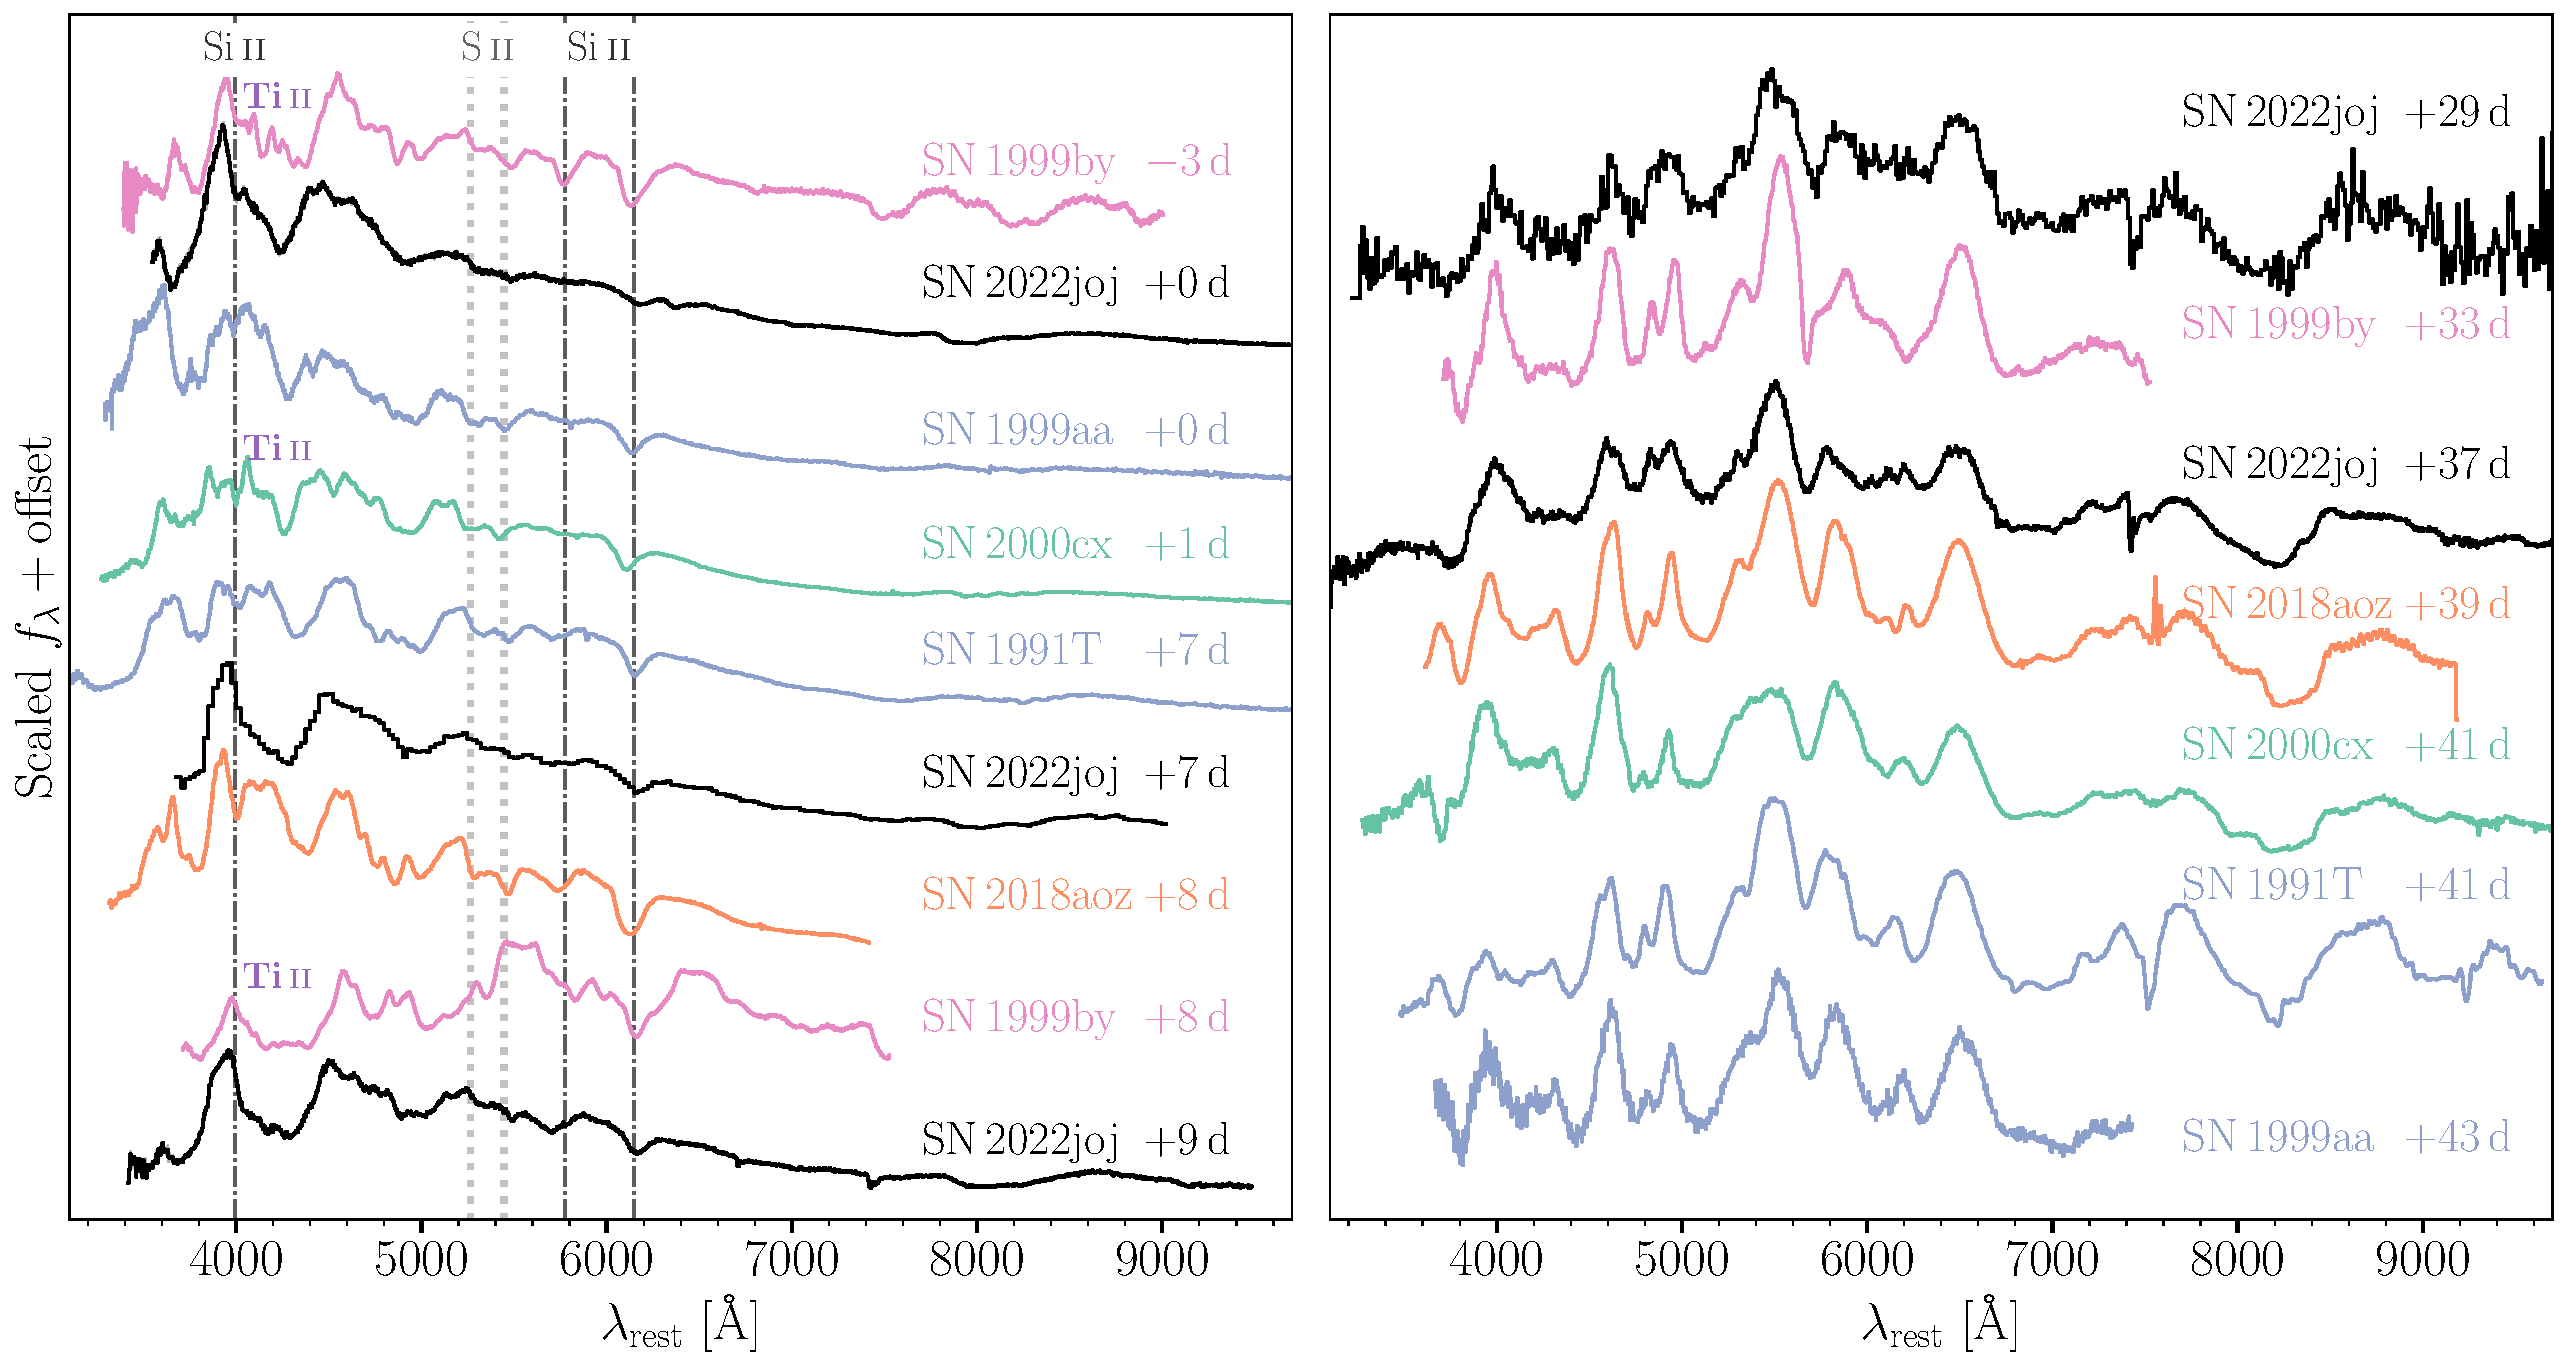
\includegraphics[width=\linewidth]{spec_comp.pdf}
    \caption{Optical spectra of \sn\ (black) and (i) a subluminous SN\,Ia, SN\,1999by (magenta), (ii) two overluminous SNe\,Ia, SN\,1991T and SN\,1999aa (blue), (iii) the peculiar SN\,2000cx (green), and (iv) a normal SN\,Ia with a red color at early timse, SN\,2018aoz (orange), near maximum brightness (left panel) and a month after maximum (right panel). The dash-dotted lines correspond to wavelengths of three \ion{Si}{2} lines (4128\,\r{A}, 5972\,\r{A}, and 6355\,\r{A}), while the dotted lines correspond to the wavelengths of the \ion{S}{2} W-trough (both assuming an expansion velocity of 10,000\,\kms). \ion{Ti}{2} has been identified from the spectra of SN\,1999by and SN\,2000cx at around $\sim$4200\,\r{A}, and the corresponding features are labeled \chang{is there a paper the confirms \ion{Ti}{2} in 00cx?}. Spectra were downloaded from WiseREP \chang{REF}, with the following original data sources: SN\,1991T, SN\,1999aa, and SN\,2000cx -- \citet{Silverman_UCBIa_2012}; SN\,1999by -- \citet{Matheson_cfaIa_2008}; SN\,2018aoz -- \citet{Ni_18aoz_2023}.}
    \label{fig:spec_comp}
\end{figure*}
\begin{figure*}
    \centering
    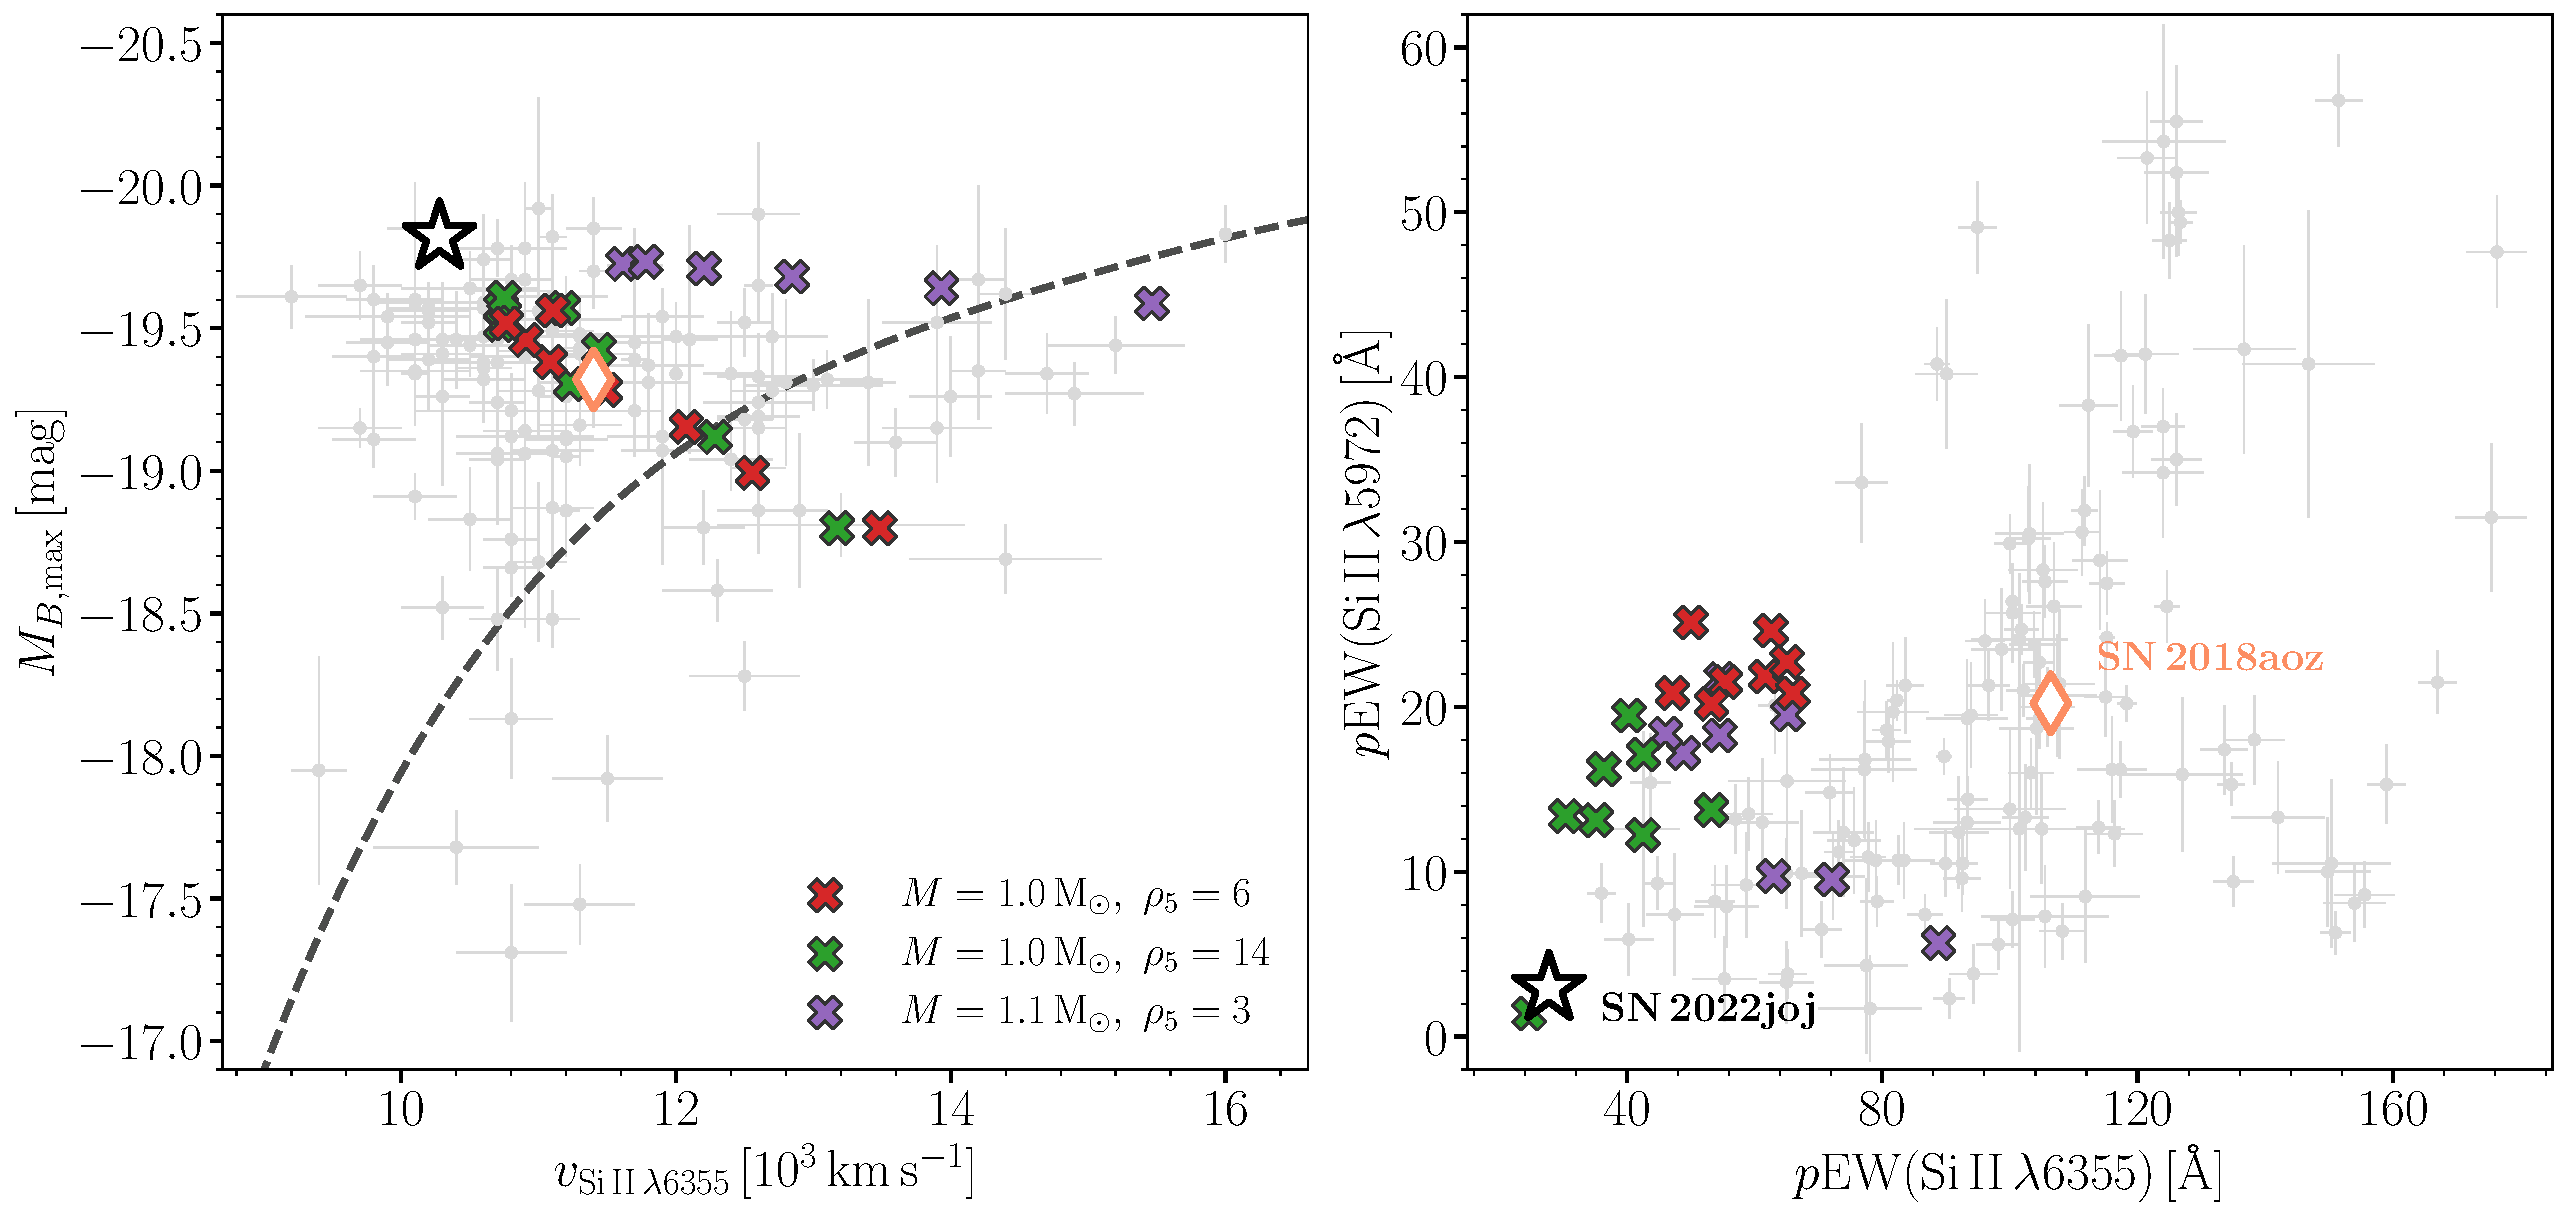
\includegraphics[width=\linewidth]{phase_space.pdf}
    \caption{\sn\ (black star) as an overluminous SN\,Ia marked by its shallow \ion{Si}{2} features. \textit{Left:} the $B$-band absolute magnitude versus the expansion velocity of \ion{Si}{2} $\lambda$6355 at maximum brightness. \textit{Right:} the pseudo-equivalent width ($p$EW) of the two \ion{Si}{2} lines, \ion{Si}{2} $\lambda\lambda$5972, 6355, at maximum brightness. The grey dots show normal SNe\,Ia from \citet{Zheng_2018} and \citet{Burrow_2020}. The colored $\times$ symbols show different 2D DDet \chang{I can't remember what we did in 20byg, but I thought we avoided DDet since it can also be interpreted as delayed detonation?} models from \citet{Shen_2D_2021}. For each model, multiple symbols are shown to summarize the effect of different viewing angles, from $\mu = -0.93$ to $\mu=+0.93$ \chang{$\mu, \rho_5, M$ all need to be explained in the caption, especially because this comes up before you describe the models in Ken's paper - you can add ``see text for more details'' but $\rho$ is impossible to understand right now}. Parameters of the potential DDet normal SN\,Ia, SN\,2018aoz \chang{REF}, are also overplotted as an orange diamond. \chang{Dashed line is not explained in this caption}}
    \label{fig:phase_space}
\end{figure*}

In Figure~\ref{fig:spec_seq}, we show the optical spectral sequence of \sn. The $-12$\,d spectrum exhibits prominent absorption lines associated with \ion{Si}{2} $\lambda$6355 and \ion{Ca}{2} IRT (this spectrum was obtained and posted on TNS by \citealt{Newsome_2022TNSCR}). It also shows a strong suppression of flux blueward of $\sim$5000\,\r{A}, confirming the unusually red photometric colors at early times. Near maximum brightness, the two SEDM spectra show a very blue continuum between $\sim$5000--8000\,\r{A} with shallow absorption features, indicating a high photometric temperature. \ion{Si}{2} $\lambda\lambda$5972, 6355 lines, the \ion{S}{2} W-trough, and \ion{Ca}{2} IRT are detectable but not prominent. A wide, asymmetric absorption feature appears between $\sim$4000--4500\,\r{A} (the 4200\,\r{A} features hereafter). There is a break on the blue edge of this feature which could be associated with \ion{Si}{2} $\lambda$4128 that is widely seen in other SNe\,Ia. However, the spectra of most normal and overluminous 99aa-like/91T-like SNe\,Ia show another peak at $\sim$4100--4200\,\r{A} redward of a narrow \ion{Si}{2} $\lambda$4128 feature, which is absent in the spectra of \sn \chang{can you point to a figure to clarify what is meant in this case}. The 4200\,\r{A} features become even wider and deeper in the ALFOSC spectrum at $\sim$$+9$\,days. Weeks after the maximum, in the FLOYDS spectrum ($+29$\,days) and the LRIS spectrum ($+36$\,days), the bottom of the 4200\,\r{A} features becomes flat, reminiscent of the Ti-trough in the subluminous SN\,1991bg-like \citep[91bg-like;][]{Filippenko_91bg_1992,Leibundgut_91bg_1993}. The nebular-phase spectra are dominated by [\ion{Fe}{2}], [\ion{Fe}{3}], and [\ion{Co}{3}] emission lines, but the [\ion{Fe}{2}] features (e.g, the complex around $\sim$7300\,\r{A}) are weaker than in other SNe\,Ia, suggesting that the ejecta remain highly ionized. The nebular spectra are discussed in detail in Section~\ref{sec:disc_nebular}.

% 4200 A
In Figure~\ref{fig:spec_comp}, we compare maximum light and transition phase spectra of \sn\ to other SNe\,Ia. Around peak, the blue continuum and shallow absorption features in \sn\ are similar to overluminous objects, including SN\,1991T, SN\,1999aa, and SN\,2000cx. The asymmetric 4200\,\r{A} features are not seen in SN\,1991T or SN\,1999aa, while in SN\,2000cx, a similar (but narrower) absorption feature is interpreted as high velocity \ion{Ti}{2} \citep{Branch_00cx_2004}. The 4200\,\r{A} features are actually much more similar to the well-known Ti-trough that is ubiquitous in subluminous 91bg-like objects, e.g., SN\,1999by \citep{Arbour_1999}. Prior to the peak, SN\,1999by also shows this asymmetric absorption at about the same wavelength. In 91bg-like SNe, this absorption feature becomes more prominent with a nearly flat-bottom trough about a week after maximum. This absorption is caused by a blend of multiple IGEs dominated by \ion{Ti}{2} \citep{Filippenko_91bg_1992,Mazzali_1997}. It remains prominent in the spectrum up to one month after maximum. Similarly, we find that this trough is prominent in the spectra of \sn\ at $+29$\,days and $+36$\,days. Other normal/overluminous SNe\,Ia, unlike \sn, all exhibit a dip around $\sim$4500\,\r{A}. Aside from the 4200\,\r{A} features, \sn\ is otherwise entirely dissimilar to 91bg-like objects, which are $\gtrsim$2\,mag fainter at peak and exhibit much stronger \ion{Si}{2}, \ion{Ca}{2} and \ion{O}{1} absorption from a cooler line-forming region \citep{Filippenko_91bg_1992}. The Ti-trough in 91bg-like SNe is interpreted as the result of a low photospheric temperature \citep{Mazzali_1997}. Whether the 4200\,\r{A} features in \sn\ are dominated by \ion{Ti}{2} absorption is unclear.

% shallow silicon
\sn\ also shows remarkably shallow \ion{Si}{2} absorption at maximum brightness. Following the techniques elaborated in \citet{Liu_20jgb_2023} \chang{would it make sense to also point to Maguire+14 since the method is adapted from that}, we fit the \ion{Si}{2} \chang{and \ion{Ca}{2} IRT} features with multiple Gaussian profiles. In Table~\ref{tab:vel_EW} we list the estimates of the expansion velocities and the pseudo-equivalent widths ($p$EWs) of the major absorption lines from $\sim$$-12$\,days to $\sim$$+9$\,days. \chang{somewhere you need to define the acronyms HVF and PVF} In Figure~\ref{fig:phase_space} we show the peak absolute magnitude in $B$ band vs.\ the velocity and $p$EW of \ion{Si}{2} for \sn\ and a sample of normal SNe\,Ia from \citet{Zheng_2018} and \citet{Burrow_2020}. Figure~\ref{fig:phase_space} highlights that \sn\ is slightly overluminous with a relatively low \ion{Si}{2} $\lambda$6355 expansion velocity (hereafter $v_\mathrm{Si}$ \chang{should this be $v_\mathrm{Si\,II}$?}). The \ion{Si}{2} $\lambda$5972 and \ion{Si}{2} $\lambda$6355 $p$EWs in \sn\ are lower than most normal SNe\,Ia. In fact, \sn\ sits at the extreme edge of the shallow-silicon group proposed in \citet{Branch_2006}, which mainly consists of overluminous 91T-like/99aa-like objects. This is consistent with the high luminosity and the blue color of \sn\ at maximum light, since a high photometric temperature promotes the average ionization level of Si \chang{do you mean higher temperatures result in higher ionization?}, reducing the abundance of singly ionized atoms. Interestingly, the $p$EW of \ion{Si}{2} $\lambda$6355 near peak is significantly lower than that in the first spectrum. In typical 91T-like/99aa-like objects, the \ion{Si}{2} features are weak or undetectable at early times because the ejecta are even hotter, and only start to emerge around maximum light \citep{Filippenko_91T_1992}. In the early spectrum of \sn, in contrast, stronger absorption features from singly ionized Si and Ca indicate a cooler line-forming region at early times compared to maximum brightness. 

In conclusion, the spectral evolution of \sn\ shows some similarities to 91T-like/99aa-like objects, as well as peculiarities \chang{I've removed the word exotic - for me this would indicate something that has never been seen before}. A reasonable model to explain \sn\ needs to reproduce (i) a strong suppression in flux blueward of $\sim$5000\,\r{A} at early times followed by a rapid evolution to blue colors; (ii) the seemingly contradictory observables at peak, namely the tentative \ion{Ti}{2} features and the blue continuum/shallow \ion{Si}{2} feature at maximum, which separately indicate low and high photometric temperatures, respectively.

\section{Discussion} \label{sec:discussion}
\subsection{Models} \label{sec:model}

\chang{I think we should be more descriptive than just models for this section}

\begin{figure*}
    \centering
    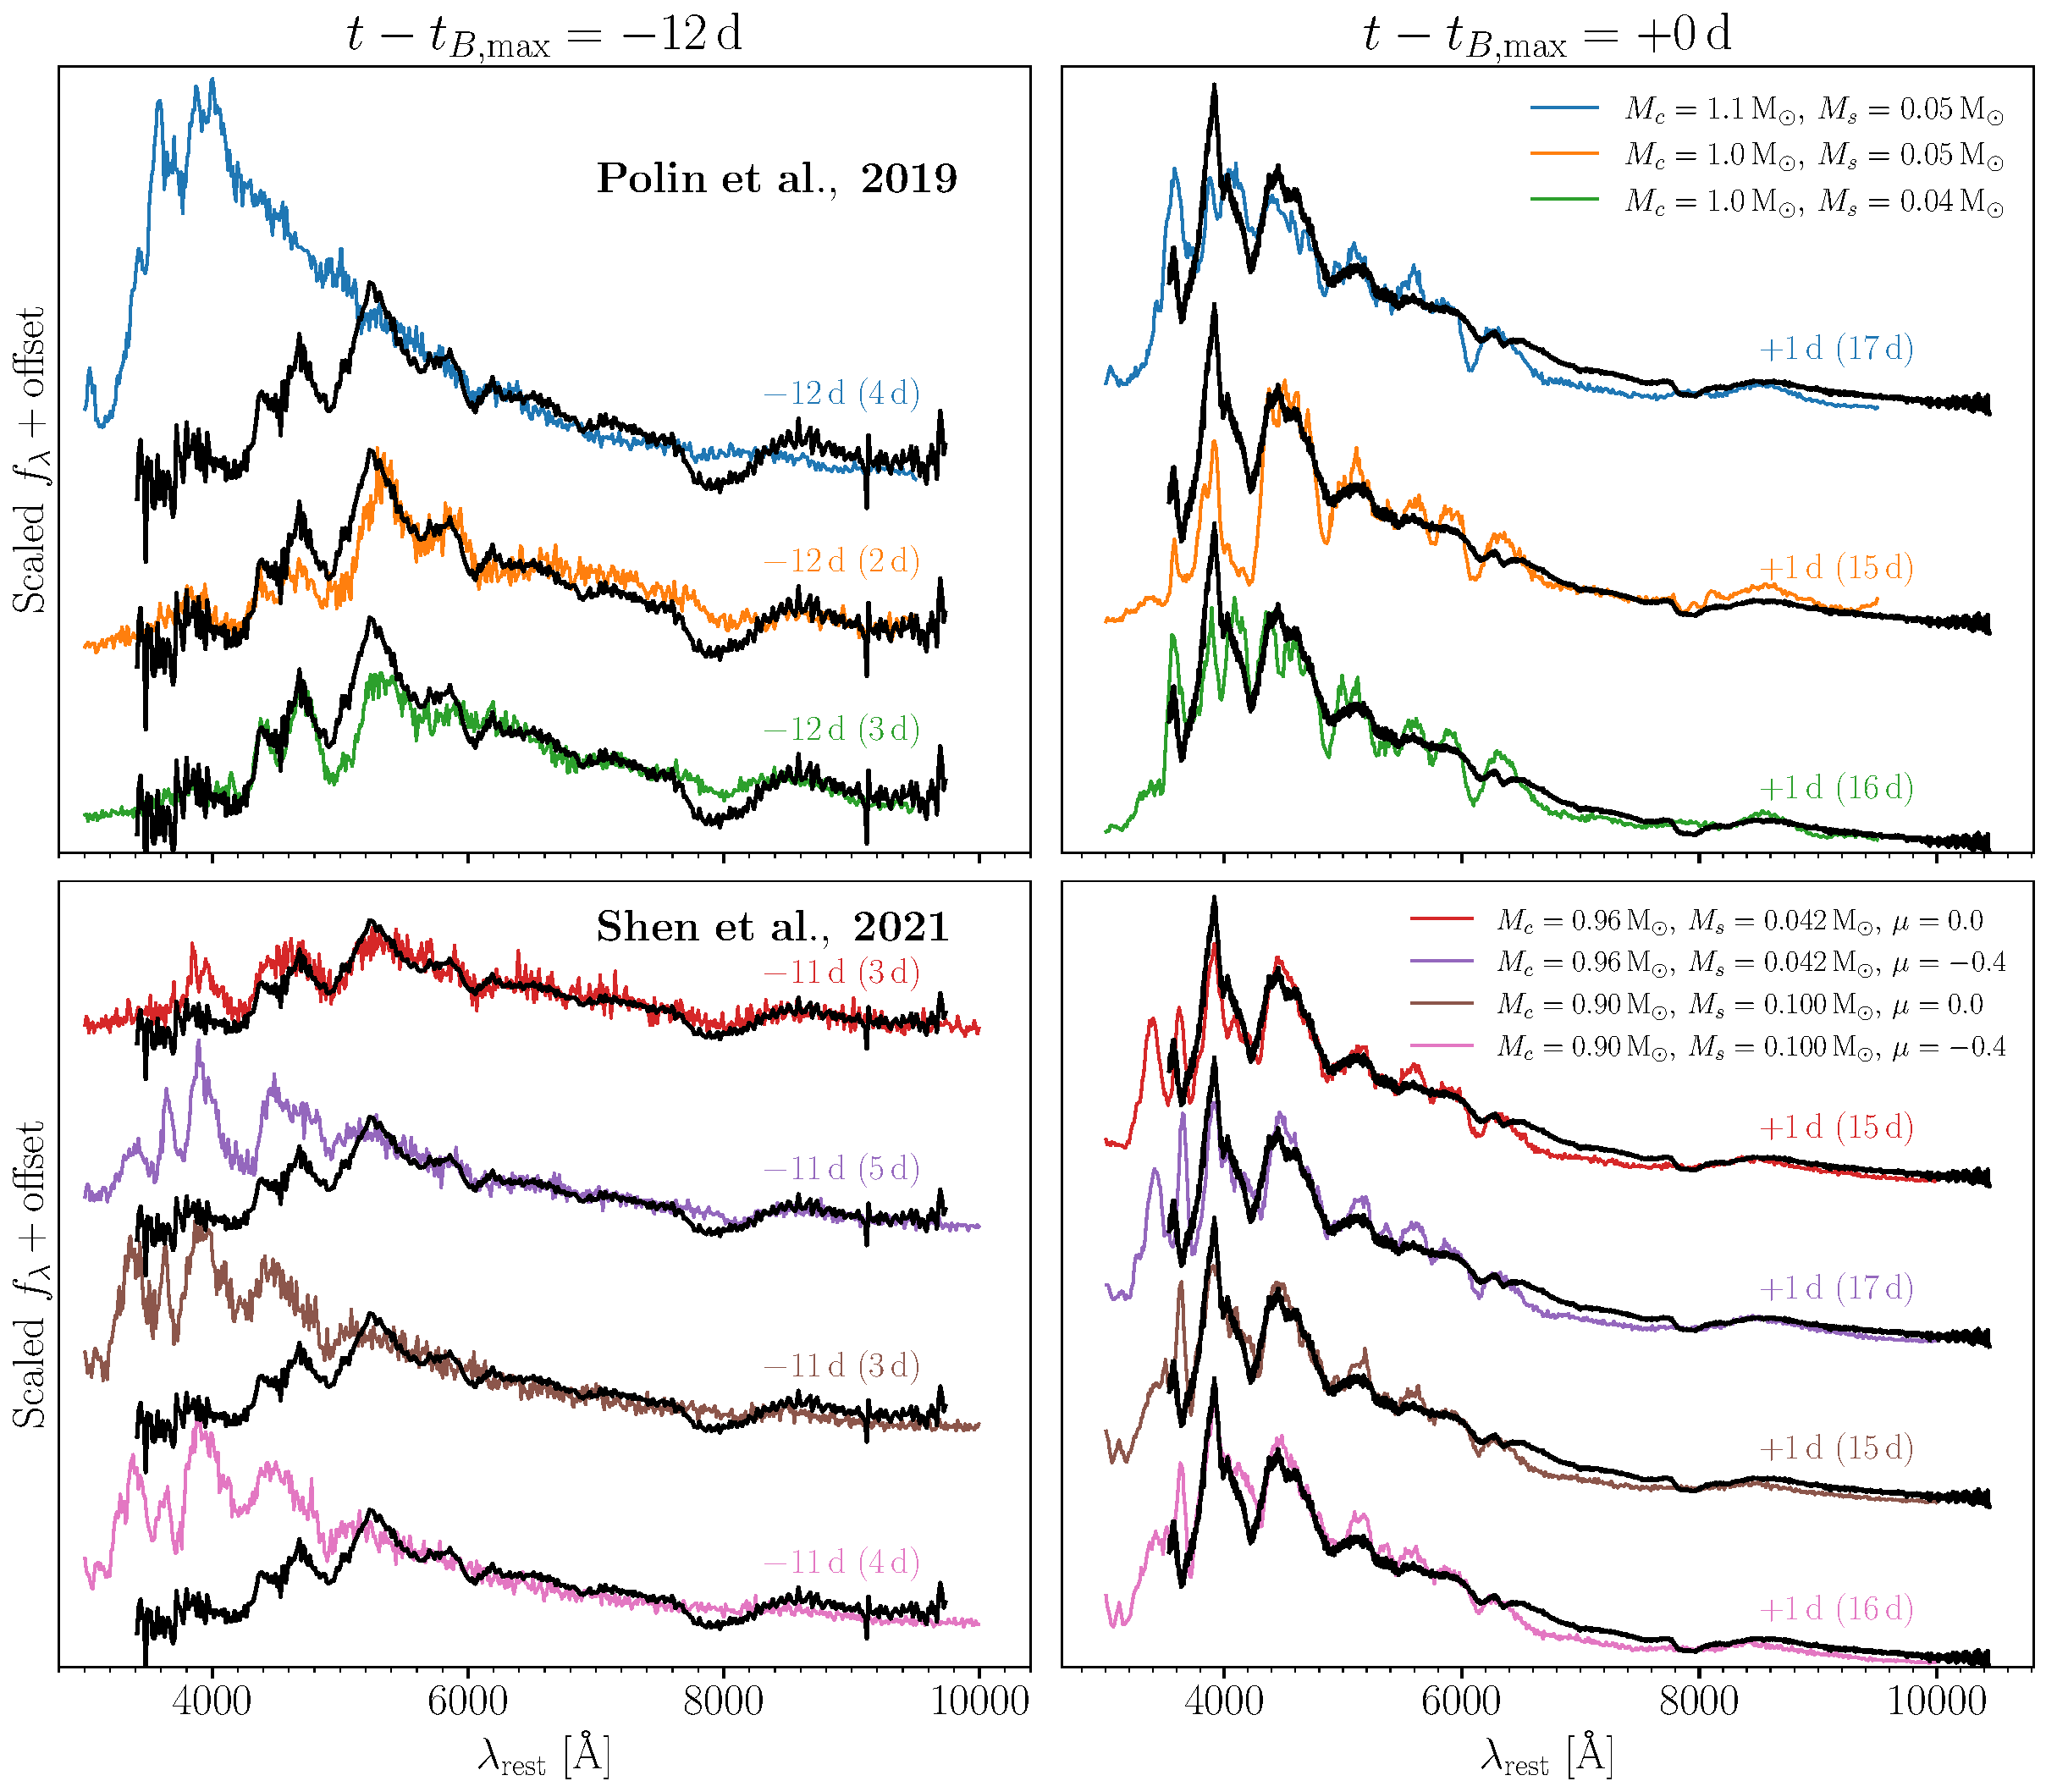
\includegraphics[width=\linewidth]{model_comparison_spec.pdf}
    \caption{Comparisons of an early spectrum ($\sim$$-12$\,days) and a maximum-light spectrum ($\sim$$+2$\,days) of \sn\ (black) with two sets of DDet models at corresponding phases. \textit{Top:} results of 1D hydrodynamical simulations from \citet{polin_observational_2019} with a variety of core masses ($M_c$) and shell masses ($M_s$). \textit{Bottom:} results of 2D hydrodynamical simulations from \citep{Shen_2D_2021} with different total masses ($M$), densities at the bottom of the helium shell ($\rho_5$ in units of $10^{5}\,\mathrm{g\,cm^{-3}}$), and viewing angles ($\mu$ defined as the cosine of the polar angle relative to the point where the helium-shell detonation occurs). A Galactic extinction of $E(B-V)_\mathrm{MW}$ has been applied to each synthetic spectrum.}
    \label{fig:model_spec}
\end{figure*}


There are several physical mechanisms that can produce blue colors during the early evolution of SNe\,Ia, including: heating of the SN ejecta following the decay of radioactive $^{56}$Ni, interaction of the SN ejecta with a nondegenerate companion \citep{Kasen_2010}, collisions between the SN ejecta and circumstellar material \citep[e.g.,][]{Piro_2016}, strong mixing that surfaces $^{56}$Ni to the outermost layers of the ejecta \citep[e.g.,][]{Piro_2013,Magee_2020}, and/or via the production of radioactive isotopes in the detonation of a He shell on the surface of the exploding white dwarf \citep[e.g.,][]{polin_observational_2019}. \chang{I'm not perfectly happy with this paragraph, but I think it's a little better to ground these ideas in theory papers rather than observations since things like 2012cg are interpretation dependent.}

% Most SNe\,Ia exhibit a blue color shortly after explosion as the ejecta remain hot in this phase. In addition, when there is an external energy source (e.g., shocks), the SN can show an excess in flux in the early light curves that appears even bluer. A non-negligible fraction of SNe\,Ia exhibit a blue flux excess \citep{Deckers_2022}. Interactions of the ejecta with either a non-degenerate companion star \citep{Cao_14atg_2015,Marion_12cg_2016,Hosseinzadeh_17cbv_2017} or some dense circumstellar material \citep{Jiang_20hvf_2021,Dimitriadis_21zny_2023} could produce such a flux excess during shock cooling. Other scenarios include the presence of $^{56}$Ni in the outermost ejecta due to mixing \citep{Piro_2013,Magee_2020}, or as the products in the detonation of a helium shell \citep{polin_observational_2019}.

On the other hand, there are few proposed scenarios that can produce red colors up to a week after explosion, as is the case of \sn. If the newly synthesized $^{56}$Ni is strongly confined to innermost SN ejecta, then a SN may remain red for several days after explosion as the heating diffuses out towards the photosphere \citep{Piro_2016}. Even the most confined $^{56}$Ni configuration considered in \citet{Piro_2016} converges to blue colors, similar to explosions with more extended $^{56}$Ni distributions, within $\sim$6\,d after explosion. \sn\ is observed to have very red colors $\sim$7\,d after $t_\mathrm{fl}$ (meaning more than 7\,d after explosion, since SNe\,Ia have a ``dark phase'' before photons diffuse out of the ejecta; \citealt{Piro_2013}). We do not know of any multidimensional explosion models that fail to produce any $^{56}$Ni mixing within the ejecta, and therefore disfavor this model.

% If the $^{56}$Ni synthesized at the center of the WD is not mixed with the outer layers and remains confined, the outer ejecta, where the $^{56}$Ni heating has yet to reach, will quickly cool down as they expand adiabatically at early times \citep{Piro_2016}. In the model with no $^{56}$Ni in \citet{Piro_2016}, for the $\sim$6\,days after the explosion the SN is expected to show an extremely red $B-V$ color (see their Figure~8), before the photosphere moves in to where the ejecta have been significant heated up by $^{56}$Ni. However, models with different degrees of mixing appear similar after the first $\sim$6\,days. In addition, models with a low degree of mixing are expected to have a ``dark phase'' \citep{Piro_2013} between the explosion and the first light of $\sim$1--5\,days, which roughly accounts for the escaping timescale of the photons emitted by the $^{56}$Ni underneath through diffusion. If the progenitor of \sn\ really has an extremely confined $^{56}$Ni distribution, then when we had our first color measurement $\sim$7\,days after \tfl, the time since the explosion could be even longer, say, $\sim$10\,days. At this phase, even the model with the most confined $^{56}$Ni distribution in \citet{Piro_2016} has turned into a normal blue color, while we still see an unusually red color in \sn. On the other hand, it has also been shown in \citet{Piro_2016} that the early light curves of the normal object SN\,2011fe is consistent with a non-negligible level of $^{56}$Ni mixing in the ejecta. It remains to be questioned whether there is an explosion scenario in which $^{56}$Ni does not get mixed at all.

Alternatively, in the DDet scenario, a layer of iron-group elements (IGEs) in the ashes of the helium shell can produce significant opacity in the outer layers of the bulk ejecta, producing a red color \citep{polin_observational_2019}. This scenario has been proposed for a few SNe with red colors at early times, including SN\,2016jhr \citep{jiang_16jhr_2017} and SN\,2018aoz \citep{Ni_2022}. In Figure~\ref{fig:model_spec} we compare the spectra of \sn\ at $\sim$$-12$\,days and near maximum light with 1D DDet models from \citet{polin_observational_2019} and 2D DDet models from \citet{Shen_2D_2021}. To create synthetic spectra, both models use \texttt{Sedona}, multi-dimensional radiative transfer simulator that assumes local thermodynamical equilibrium (LTE).

In the 1D models, the most important model parameters are the mass of the C/O core ($M_c$) and the mass of the helium shell ($M_s$). The maximum luminosity depends on the amount of $^{56}$Ni synthesized in the explosion, which is predominantly determined by the total progenitor mass ($M_c+M_s$) in 1D models \citep{polin_observational_2019}. We find that the maximum brightness in $B$ band ($M_{B,\mathrm{max}}=-19.82$\,mag) is reproduced by the 1D models with relatively massive progenitors ($\sim$1.2\,$\mathrm{M_\odot}$). However, models with such massive progenitors tend to produce blue, featureless spectra at early times (e.g., the $M_c=1.1\,\mathrm{M_\odot}$, $M_s=0.05\,\mathrm{M_\odot}$ model in Figure~\ref{fig:model_spec}), inconsistent with the observations. Less massive models provide a better match to the line-blanketing seen in the early spectra, but fail to reproduce the maximum brightness as well as the 4300\,\r{A} \chang{wasn't this called 4200 earlier?} features in the observed spectra. The 1D models overestimate the $p$EW and the expansion velocity of the \ion{Si}{2} $\lambda$6355 line at peak. We overplot the theoretical $M_{B,\mathrm{max}}$-$v_\mathrm{Si}$ relation of 1D DDet models across a spectrum of progenitor masses in \citet{polin_observational_2019} as the dashed black curve in the left panel of Figure~\ref{fig:phase_space}, which is not in agreement with the properties of \sn. \chang{A couple more details are needed here - is that sequence for high mass shells? low mass shells? it does not capture every single model in Abi's paper.}

While the 1D models do not fully reproduce the observed properties of \sn, some of these tensions can be resolved when considering viewing angle effects in multi-dimensional models. In Figure~\ref{fig:phase_space} we also show the properties of three 2D DDet models from \citet{Shen_2D_2021}. The selected models have different total progenitor masses $M$ and densities at the bottom of the helium shell $\rho_5$ (in units of $\mathrm{10^5\,g\,cm^{-3}}$). For these models, we obtain the \ion{Si}{2} line properties using the same fitting techniques as in Section~\ref{sec:analysis_spec}. We again find that more massive progenitors generally lead to more luminous SNe, but different viewing angles produce significantly different spectral properties. In the plot, the cosine value of the polar angle relative to the point of helium detonation, $\mu$, ranges from $+0.93$ (near the helium detonation) to $-0.93$ (opposite to the helium detonation). When the SN is observed along a line of sight closer to the detonation point in the shell (greater $\mu$), it will appear fainter at maximum brightness and show a higher line velocity in \ion{Si}{2} $\lambda$6355. For a relatively high progenitor mass ($\gtrsim$$1.1\,\mathrm{M_\odot}$), a high $v_\mathrm{Si}$ ($\gtrsim$$13,500$\,\kms) is predicted. However, with $\mu\lesssim0$, all the 2D models show a lower $v_\mathrm{Si}$ ($\lesssim$$12,000$\,\kms), much closer to \sn\ in the $M_{B,\mathrm{max}}$-$v_\mathrm{Si}$ phase space. Models with $\mu>0$ are more consistent with 1D model predictions. It is argued in \citep{polin_observational_2019} that high-velocity SNe that follow the dashed line in Figure~\ref{fig:phase_space} are sub-\Mch\ DDets, while SNe in the clump centered at $M_{B,\mathrm{max}}\simeq-19.5$\,mag and $v_\mathrm{Si}\simeq11,000$\,kms are likely near-\Mch\ explosions. Based on the 2D models, however, we should expect a similar number of high-velocity and normal-velocity DDet SNe\,Ia. A substantial fraction of the objects within the clump on the $M_{B,\mathrm{max}}$-$v_\mathrm{Si}$ diagram, which has been proposed to consist of mostly near-\Mch\ events, may turn out to be sub-\Mch\ DDet events viewed from certain orientations \citep{Shen_2D_2021} \chang{this sentence feels redundant - consider cutting?}. SN\,2018aoz is a DDet candidate that, like \sn, exhibits early red colors before evolving to normal luminosity and blue colors \citep{Ni_2022}. Interestingly, SN\,2018aoz also resides in the high-luminosity, low-velocity clump in the $M_{B,\mathrm{max}}$-$v_\mathrm{Si}$ space \citep{Ni_18aoz_2023}, and thus, it too may be an example of a DDet SN\,Ia viewed from the opposite hemisphere opposite from helium detonation.

%SN\,2018aoz shows an early flux excess in $V$ within the first few days since its first light, during which the $B$-band flux is suppressed. The resulting red $B-V$ color is consistent with the predictions of a 1D DDet model with $M_c=1.05\,\mathrm{M_\odot}$ and $M_s=0.01\,\mathrm{M_\odot}$ \citep{Ni_2022}. Near maximum

In the bottom panels of Figure~\ref{fig:model_spec} we show three 2D DDet models with a total progenitor mass of $\sim$$1\,\mathrm{M_\odot}$ from \citet{Shen_2D_2021}. These models, particularly the $mu = -0.67$ ones \chang{double check this}, qualitatively match the observed spectra at maximum light. The $\rho_5=6$ model has a helium shell of $\sim$0.05$\,\mathrm{M_\odot}$. We find that when $\mu=0$ (viewed from the equator), the model predicts a reasonable level of line blanketing in the blue side of the spectrum at early times (lower left panel of Figure~\ref{fig:model_spec}). Near maximum brightness, the model also reproduces the overall shape of the observed spectrum, though the strength of nearly all the absorption lines (4200\,\r{A} features, \ion{S}{2}, and \ion{Si}{2}) is overestimated. $v_\mathrm{Si}$ is also overestimated ($\sim$12,000\,\kms). When viewed from the opposite hemisphere from the helium detonation point (e.g., $\mu=-0.67$), the model yields an asymmetric profile of 4200\,\r{A} features as a blend of \ion{Ti}{2}, \ion{Fe}{2}, and \ion{Co}{2} lines that matches the observations better. The \ion{Si}{2} features are also predicted to be shallower, though still not as shallow as that in the observations. Nonetheless, the spectra at early times are expected to be much bluer than the observations. The $\rho_5=14$ model has a thicker helium shell ($\sim$0.1\,$\mathrm{M_\odot}$), and produces even shallower and slower-expanding \ion{Si}{2} features at maximum brightness. This is in agreement with the trend observed in the right panel of Figure~\ref{fig:phase_space}: models with a thicker helium shell tend to exhibits shallower \ion{Si}{2} features. However, the \ion{Ti}{2} absorption is not sufficiently strong. The level of line-blanketing blueward of $\sim$5000\,\r{A} is also underestimated at early times. In addition, all three models, which have $M_{B,\mathrm{max}}\simeq -19.3$\,mag, are not as bright as \sn. While a more massive 2D model may provide a better match to the observations, unfortunately, there are only two models in \citet{Shen_2D_2021} with progenitor masses $>1\,\mathrm{M_\odot}$, and both have thin helium shells ($\lesssim$$0.01\,\mathrm{M_\odot}$). These models therefore cannot reproduce the red color at $\sim$$-12$\,days or the remarkable 4200\,\r{A} features at peak.

\chang{somewhere it should be emphasized that none of the models considered here were developed to EXPLAIN 22joj. Instead they are from existing papers and therefore do not have any tuning specifically for this event.}

While none of the models presented here provide a strong match to \sn\ at every phase, we draw the broad conclusion that the spectroscopic properties of \sn\ are qualitatively consistent with a sub-\Mch\ WD ($\gtrsim$1.0\,$\mathrm{M_\odot}$) DDet viewed opposite from the shell ignition point. Observers from such a viewing angle would observe strong absorption features in the blue portion of the spectrum dominated by \ion{Ti}{2} and IGEs as well as relatively shallow and slowly-expanding \ion{Si}{2} lines in the red portion. Customized models specifically tuned for \sn\ may reproduce all the observed features simultaneously, and we suggest more 2D DDet simulations be performed. Additional improvements can be made via an improved handling of the radiative transfer \citep[e.g., non-LTE effects; see][]{Shen_NLTE_2021}.

\subsection{The 7300\,\r{A} Region in Nebular-phase Spectra}
\label{sec:disc_nebular}
\begin{figure*}
    \centering
    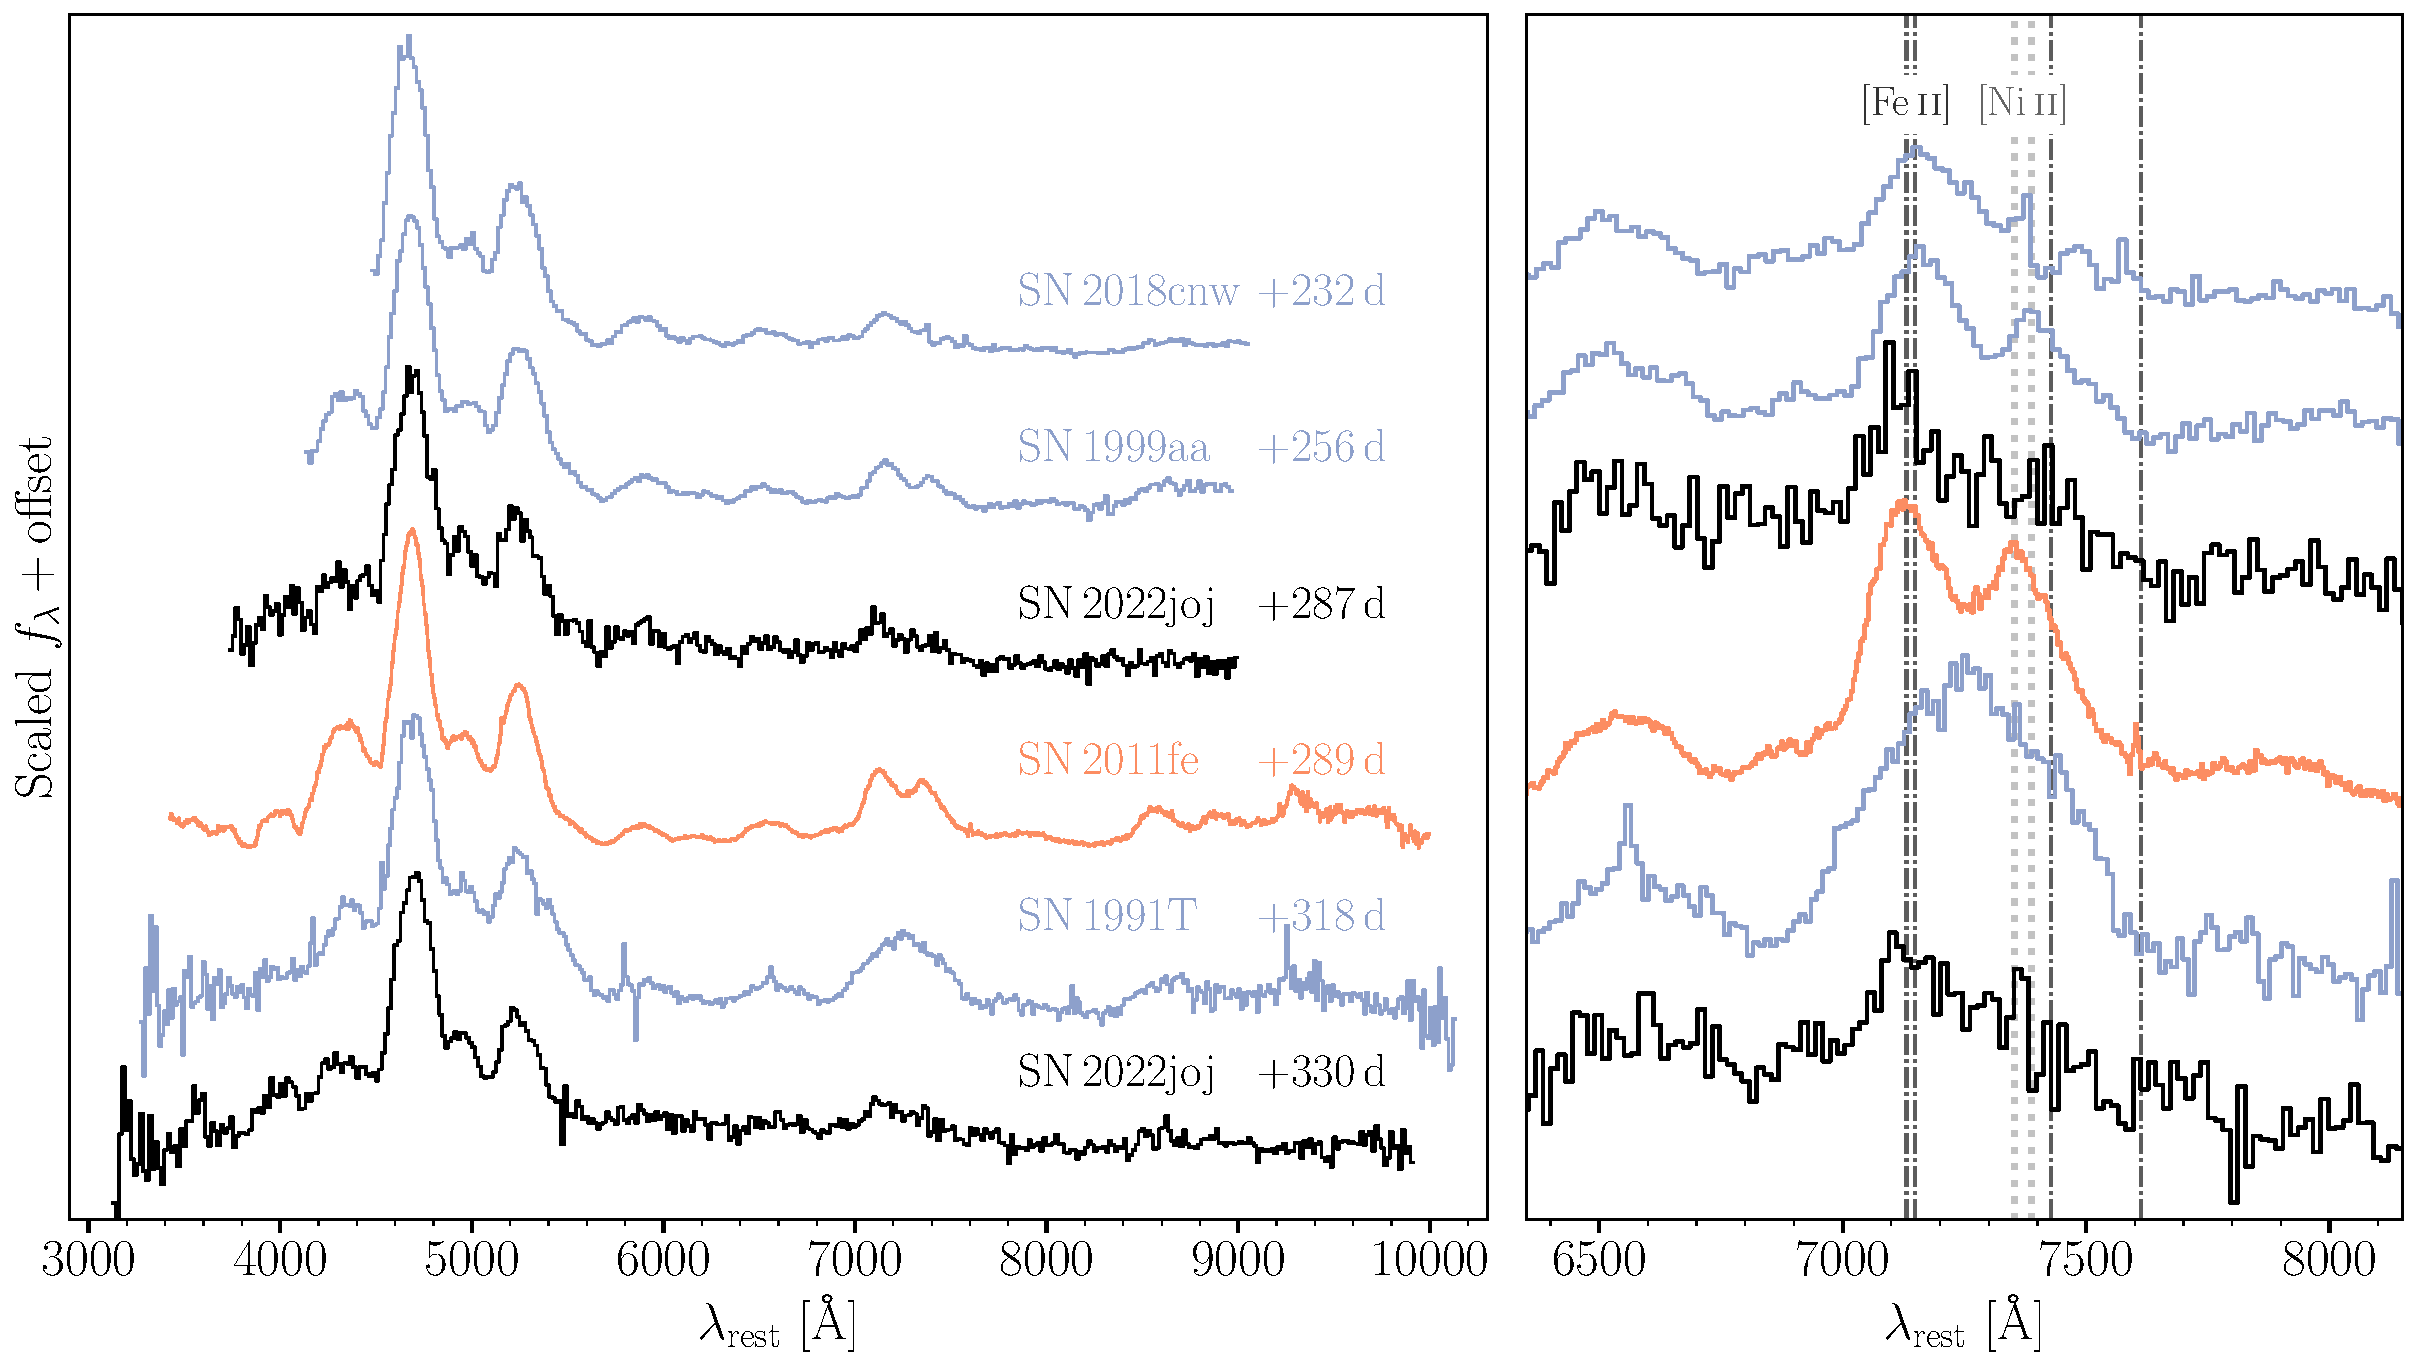
\includegraphics[width=\linewidth]{spec_comp_nebular.pdf}
    \caption{Nebular-phase spectra of \sn\ (black), three overluminous SNe\,Ia (blue), SN\,1991T, SN\,1999aa, and SN\,2018cnw, and a normal SN\,Ia (orange), SN\,2011fe. The right panel zooms in on the features around 7300\,\r{A}. The flux has been normalized to the [\ion{Fe}{3}] features around 4700\,\r{A}. The dash-dotted lines correspond to wavelengths of four [\ion{Fe}{2}] lines (7155\,\r{A}, 7172\,\r{A}, 7453\,\r{A}, and 7638\,\r{A}), while the dotted lines correspond to the wavelengths of two [\ion{Ni}{2}] lines (7378\,\r{A}, 7412\,\r{A}), both blueshifted by 1000\,\kms.}
    \label{fig:nebular_spec}
\end{figure*}
\begin{figure}
    \centering
    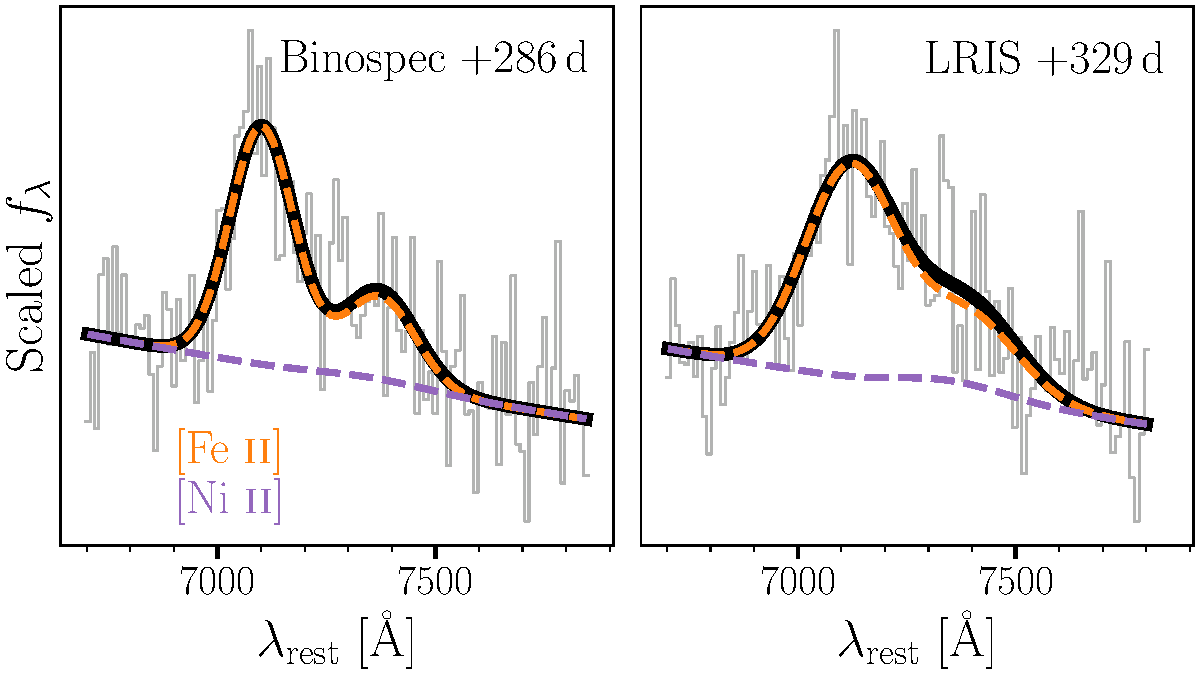
\includegraphics[width=\linewidth]{Fe_Ni.pdf}
    \caption{Fits to the 7300\,\r{A} region containing [\ion{Fe}{2}] and [\ion{Ni}{2}] features are consistent with a low \ion{Ni}{2} abundance. The observed spectra are shown in grey. The dashed lines correspond to the models of [\ion{Fe}{2}] (orange) and [\ion{Ni}{2}] (purple) features. For the model parameters we adopt the mean values of their posterior distributions. The black solid lines are the overall models.}
    \label{fig:Fe_ni}
\end{figure}

In Figure~\ref{fig:nebular_spec} we compare the two nebular-phase spectra of \sn\ with the overluminous SNe\,Ia (SN\,1991T, SN\,1999aa, and SN\,2018cnw) and the normal luminosity SN\,2011fe.

Compared to other SNe\,Ia, the nebular spectra of \sn\ show a relatively low flux ratio between the complex at $\sim$7300\,\r{A} (hereafter the 7300\,\r{A} features) and the [\ion{Fe}{3}] 4700\,\r{A} features. This suggests high ionization in the ejecta \citep{Wilk_2020}. In addition to the smaller flux ratio, the profile of the 7300\,\r{A} features in \sn\ is also distinct from other SNe. Most of SNe\,Ia show a bimodal structure in their 7300\,\r{A} features \citep[e.g.,][]{Graham_2017,Maguire_2018}. The bluer peak is dominated by [\ion{Fe}{2}] $\lambda\lambda$7155, 7172, while [\ion{Ni}{2}] $\lambda\lambda$7378, 7412 usually have non-negligible contributions to the redder peak (see Figure~\ref{fig:nebular_spec}). The bimodal morphology is prominent in the spectra of SN\,1999aa and SN\,2011fe. SN\,1999T is well-known for its broader emission lines in the nebular phase, so the composition of the 7300\,\r{A} features is ambiguous. In the spectra of \sn\ and SN\,2018cnw, however, the redder peak is absent and the 7300\,\r{A} features show an asymmetric single peak, which seems to indicate a low abundance of Ni in the ejecta.

% We mainly focus on the complex at $\sim$7300\,\r{A} (here after the 7300\,\r{A} features) that is usually dominated by [\ion{Fe}{2}] and [\ion{Ni}{2}], although in some peculiar SNe\,Ia, [\ion{Ca}{2}] $\lambda\lambda$7291, 7324 emissions are also detected \cite[e.g.,][]{Siebert_2020} \chang{There is a long history of Ca-rich objects that should be mentioned here - like Kishalay's paper, and the many references therein}. Both spectra of \sn\ show relatively low flux ratio between the 7300\,\r{A} features and the [\ion{Fe}{3}] 4700\,\r{A} features, compared to other SNe\,Ia. This suggests high ionization in the ejecta \citep{Wilk_2020}. The profile of the 7300\,\r{A} features in \sn\ is also distinct from others. Most of SNe\,Ia show a bimodal structure in their 7300\,\r{A} features \citep[e.g.,][]{Graham_2017,Maguire_2018}. The bluer peak is dominated by [\ion{Fe}{2}] $\lambda\lambda$7155, 7172, while [\ion{Ni}{2}] $\lambda\lambda$7378, 7412 usually have non-negligible contributions to the redder peak (see Figure~\ref{fig:nebular_spec}). The bimodal morphology is prominent in the spectra of SN\,1999aa and SN\,2011fe. SN\,1999T is well-known for its broader emission lines in the nebular phase, so the composition of the 7300\,\r{A} features is ambiguous. In the spectra of \sn\ and SN\,2018cnw, however, the redder peak is absent and the 7300\,\r{A} features show an asymmetric single peak, which seems to indicate a low abundance of Ni in the ejecta.

To investigate the relative contributions of [\ion{Fe}{2}] and [\ion{Ni}{2}] to the 7300\,\r{A} features in \sn, we model this region with multiple Gaussian emission profiles using the same technique as in Section~\ref{sec:analysis_spec}. We include four [\ion{Fe}{2}] lines (7155, 7172, 7388, 7453\,\r{A}) and two [\ion{Ni}{2}] lines (7378, 7412\,\r{A}) in the fit. For each species, the relative flux ratios of lines are fixed, whose values are adopted from \citet{Jerkstrand_2015}. For [\ion{Fe}{2}], we set $L_{7155}:L_{7172}:L_{7388}:L_{7453} = 1:0.24:0.19:0.31$, and for [\ion{Ni}{2}], we set $L_{7378}:L_{7412} = 1:0.31$. These line ratios are calculated assuming LTE, but the departure from LTE should not be significant under the typical conditions in the ejecta \citep{Jerkstrand_2015}. We allow the amplitudes of these Gaussian profiles to be either positive or negative. The velocity dispersions in different lines of each species are set to be the same. The fitted models are shown in Figure~\ref{fig:Fe_ni}, where colored curves correspond to the [\ion{Fe}{2}] and [\ion{Ni}{2}] emission adopting the mean values of the posterior distributions of model parameters sampled with MCMC \chang{priors should be mentioned whenever doing Bayes - it's find to wide and flat if that's what you've done}. In both spectra, the flux of [\ion{Ni}{2}] is consistent with 0 (${L_{\mathrm{Ni}\,\textsc{ii}}}/{L_{\mathrm{Fe}\,\textsc{ii}}}=0.04\pm0.11$ at $+286$\,days and $0.07\pm0.11$ at $+329$\,days; the flux ratios of lines are estimated with the ratios of their $p$EWs), and the 7300\,\r{A} features can be well fit with [\ion{Fe}{2}] emission only. We have also tested fitting this complex with [\ion{Ca}{2}] in addition to [\ion{Fe}{2}] and [\ion{Ni}{2}], and we find no evidence for [\ion{Ca}{2}]. \chang{here is where I'd mention some SNe\,Ia show Ca II in the nebular phase - but I don't think we HAVE to say that}

The relative abundance of Ni and Fe, which probes the mass of the progenitor WD, can be estimated via the flux ratio of their emission lines. At $>$300\,d after explosion $^{56}$Fe is the dominant isotope of Fe following the decay of $^{56}$Ni through the chain: $^{56}$Ni$\rightarrow^{56}$Co$\rightarrow^{56}$Fe. Consequently, the Fe abundance primarily depends on the yield of $^{56}$Ni. The Ni abundance, however, is sensitive to both the progenitor mass and the explosion scenario. The stable Ni isotopes ($^{58}$Ni, $^{60}$Ni, and $^{62}$Ni) are more neutron-rich compared to the $\alpha$-species $^{56}$Ni, and can only be formed in high-density regions with an enhanced electron capture rate during the explosion \citep{Nomoto_1984,Khokhlov_1991}. Consequently, SNe\,Ia from sub-\Mch\ WDs, with central densities that are lower than near-\Mch\ WDs, are expected to show a lower abundance of stable Ni isotopes \citep{Iwamoto_1999,Seitenzahl_2013,Shen_DD_2018}. 

To estimate the relative abundance of Ni and Fe, we use the equation adopted in \citet{Jerkstrand_2015} and \citet{Maguire_2018},
\begin{equation}
    \frac{L_{7378}}{L_{7155}} = 4.9\frac{n_{\mathrm{Ni}\,\textsc{ii}}}{n_{\mathrm{Fe}\,\textsc{ii}}}\exp\left(\frac{0.28\,\mathrm
    {eV}}{k_BT}\right)\frac{dc_{\mathrm{Ni}\,\textsc{ii}}}{dc_{\mathrm{Fe}\,\textsc{ii}}},
\end{equation}
where $L_{7378}/L_{7155}$ is the flux ratio of the [\ion{Ni}{2}] $\lambda$7378 to [\ion{Fe}{2}] $\lambda$7155 lines, $n_{\mathrm{Ni}\,\textsc{ii}}$ ($n_{\mathrm{Fe}\,\textsc{ii}}$) is the number density of \ion{Ni}{2} (\ion{Fe}{2}), and ${dc_{\mathrm{Ni}\,\textsc{ii}}}/{dc_{\mathrm{Fe}\,\textsc{ii}}}$ is the ratio of the departure coefficients from LTE for these two ions. Since both \ion{Ni}{2} and \ion{Fe}{2} are singly ionized species with similar ionization potentials, we assume that $n_{\mathrm{Ni}\,\textsc{ii}}/n_{\mathrm{Fe}\,\textsc{ii}}$ is a good approximation of the total Ni/Fe ratio. As is illustrated in \citet{Maguire_2018}, this assumption proves to be valid by modeling nebular phase spectra at similar phases \citep{Fransson_2015,Shingles_2022}, with the relative deviation from the ionization balance $\lesssim$20\%. We handle the uncertainties due to the unknown temperature, ratio of departure coefficients, and the ionization balance in a Monte Carlo way. We randomly generate $N=4000$ samples of the temperature (3000--8000\,K), the ratio of departure coefficients (1.2--2.4), and the ionization balance factor (0.8--1.2) assuming uncorrelated uniform distributions. These intervals are again adopted from \citet{Maguire_2018}. Combining these quantities with the samples of line profile parameters drawn with the MCMC, we obtain $N$ estimates of Ni/Fe, which are effectively drawn from its posterior distribution. The mean value of Ni/Fe is $\sim$0.004 and we obtain a 3-$\sigma$ upper limit of $\mathrm{Ni/Fe}<0.026$. Such a low Ni abundance is more consistent with the yields of sub-\Mch\ DDet scenarios \citep{Shen_DD_2018}, much lower than the expected outcomes of near-\Mch, delayed detonation models \citep{Seitenzahl_2013} or pure deflagration models \citep{Iwamoto_1999}.

We also find that the [\ion{Fe}{2}] lines are significantly blueshifted ($v_\mathrm{[Fe\,\textsc{ii}]}=-2.36\pm0.35\mathrm{\,km\,s^{-1}}$ at $+286$\,days and $-1.52\pm0.51\mathrm{\,km\,s^{-1}}$ at $+329$\,days). This is consistent with other SNe\,Ia showing low $v_\mathrm{Si}$ at maximum brightness \citep{Maeda_2010,Maguire_2018,Li_2021}, and also in qualitative agreement with the asymmetric sub-\Mch\ DDet scenarios. Specifically, along a line of sight opposite to the shell detonation point, observers would see intermediate mass elements (IMEs) with low expansion velocities, including \ion{Si}{2}. In the meantime, the IGEs at the center of the ejecta would have a bulk velocity towards the observer \citep{Fink_DD_2010,Bulla_2016}. \chang{I don't totally understand this argument can we discuss a little more.}

\section{Conclusions} \label{sec:conclusion}
We have presented observations of \sn, a peculiar, overluminous SNe\,Ia. \sn\ has an unusual color evolution, with a remarkably red $g_\mathrm{ZTF}-r_\mathrm{ZTF}$ color at early times due to continuous absorption in the blue portion of its spectral energy distribution. Absorption features observed around maximum light simultaneously suggest high (a blue continuum, shallow \ion{Si}{2} lines) and low (strong absorption around 4200\,\r{A} that may be associated with \ion{Ti}{2}) photospheric temperatures. The nebular-phase spectra of \sn\ suggest a high ionization and low Ni abundance in the ejecta, consistent with a sub-\Mch\ explosion.

The early red colors are most likely due to a layer of IGEs in the outermost ejecta as products of a helium-shell detonation, in the sub-\Mch\ DDet scenario. If the asymmetric ejecta are observed opposite from the point of He shell ignition, we find that the resultant synthetic spectra could qualitatively reproduce some of the observed properties, including (i) significant line-blanketing of flux due to IGEs at early phases; (ii) strong \ion{Ti}{2} features as well as relatively weak \ion{Si}{2} features near maximum brightness, and (iii) blueshifted [\ion{Fe}{2}] $\lambda$7155 accompanied with a relatively low expansion velocity of \ion{Si}{2} at peak. \chang{I think many will be skeptical that we have definitely shown that there is Ti II present in this SN - we should discuss this a little more} No existing DDet model can fully explain all the observational properties of \sn. As a result, it is possible that some alternative model is superior, though we find the early red colors are difficult to explain with any other alternative explosion scenario. \chang{as I write this sentence I realize we need to take a look at pulsational delayed detonations}  Future 2D models covering a finer grid of progenitor properties may answer the question if \sn\ is really a peculiar SN triggered by a DDet.\\

%We also emphasize the importance of obtaining near-infrared spectra at multiple phases for DDet candidates. After maximum brightness, the unburnt helium in the shell could produce prominent absorption features in NIR \citep[e.g., \ion{He}{1} $\lambda$10381;][]{Boyle2017_Helium}, which, if detected, would be a decisive and robust evidence for a DDet origin \citep{Dong_16dsg_2022,Liu_20jgb_2023}. During the nebular phase, the NIR spectrum will help constrain the velocities and abundances of IGEs produced in the center of the WD, carrying rich information of the progenitor properties and explosion mechanisms \citep[e.g.,][]{Maguire_2018,Flors_2020}

%If confirmed to be a DDet event, \sn\ would be the second peculiar DDet SN discovered in a dwarf galaxy with the stellar mass $\lesssim$$10^8\,\mathrm{M_\odot}$, following SN\,2020jgb \citep{Liu_20jgb_2023}, while there are $\lesssim$10 peculiar DDet candidates spotted. The stellar population properties of these faint galaxies are usually difficult to study.\\

%\begin{acknowledgements}

% \noindent {We thank the anonymous referee for a thoughtful and detailed report.} We thank Jiaxuan Li for suggesting using the HSC image for the host galaxy. We are grateful to Aishwarya Dahiwale, Jillian Rastinejad, and Yuhan Yao for the high-quality spectra they obtained. We also appreciate the excellent assistance of the staffs of the various observatories where data were obtained. K.D. acknowledges support from NASA through the NASA Hubble Fellowship grant \#HST-HF2-51477.001 awarded by the Space Telescope Science Institute, which is operated by the Association of Universities for Research in Astronomy, Inc., for NASA, under contract NAS5-26555. A.V.F. is grateful for financial support from the Christopher R. Redlich Fund and many other individual donors. K.M. is funded by the EU H2020 ERC grant No. 758638. S.S. acknowledges support from the G.R.E.A.T research environment, funded by {\em Vetenskapsr\aa det}, the Swedish Research Council, project number 2016-06012. This work was also supported by the GROWTH project \citep{Kasliwal2019} funded by the National Science Foundation (NSF) under grant 1545949.

This work is based on observations obtained with the Samuel Oschin Telescope 48-inch and the 60-inch Telescope at the Palomar Observatory as part of the Zwicky Transient Facility project. ZTF is supported by the National Science Foundation under Grant No. AST-1440341 and a collaboration including Caltech, IPAC, the Weizmann Institute of Science, the Oskar Klein Center at Stockholm University, the University of Maryland, the University of Washington, Deutsches Elektronen-Synchrotron and Humboldt University, Los Alamos National Laboratories, the TANGO Consortium of Taiwan, the University of Wisconsin at Milwaukee, and Lawrence Berkeley National Laboratories. Operations are conducted by COO, IPAC, and UW. 
SED Machine is based upon work supported by the National Science Foundation under Grant No.\ 1106171.

% This work is also based on observations made with the Nordic Optical Telescope, owned in collaboration by the University of Turku and Aarhus University, and operated jointly by Aarhus University, the University of Turku and the University of Oslo, representing Denmark, Finland and Norway, the University of Iceland and Stockholm University at the Observatorio del Roque de los Muchachos, La Palma, Spain, of the Instituto de Astrofisica de Canarias.

The W. M. Keck Observatory is operated as a scientific partnership among the California Institute of Technology, the University of California and NASA; the observatory was made possible by the generous financial support of the W. M. Keck Foundation. W. M. Keck Observatory access was supported by Northwestern University and the Center for Interdisciplinary Exploration and Research in Astrophysics (CIERA). \chang{need to cite Binospec access too}

%\end{acknowledgements}

\facility{PO:1.2m (ZTF), PO:1.5m (SEDM), FTN (FLOYDS), FTS (FLOYDS), NOT (ALFOSC), Liverpool:2m (SPRAT), Keck:I (LRIS), MMT (Binospec).}
\software{\texttt{astropy} \citep{Astropy_2013, Astropy_2018}, 
% \texttt{CASTRO} \citep{Almgren_Castro_2010}, 
% \texttt{dynesty} \citep{Speagle_dynesty_2020}, 
% \texttt{LAMBDAR} \citep{Wright2016a}, 
\texttt{matplotlib} \citep{Matplotlib_2007}, 
\texttt{NumPy} \citep{numpy_2020},
% \texttt{prospector} \citep{Johnson_prospector_2021}, 
\texttt{PyMC} \citep{pymc_2016},
\texttt{PypeIt} \citep{pypeit:zenodo}, 
\texttt{pysedm} \citep{Rigault_pysedm_2019},
\texttt{SALT3} \citep{Kenworthy_SALT3_2021},
\texttt{sncosmo} \citep{Barbary_SNCosmo_2023},
% \texttt{Python-FSPS} \citep{Conroy_2009,Conroy_2010}, 
% \texttt{scipy} \citep{Scipy_2020}.
% \texttt{seaborn} \citep{Waskom_seaborn_2021}, 
% \texttt{SEDONA} \citep{Kasen_Sedona_2006}.
}


\bibliography{SN2022joj, software, telescope}
\bibliographystyle{aasjournal}

%% This command is needed to show the entire author+affiliation list when
%% the collaboration and author truncation commands are used.  It has to
%% go at the end of the manuscript.
%\allauthors

%% Include this line if you are using the \added, \replaced, \deleted
%% commands to see a summary list of all changes at the end of the article.
%\listofchanges

\end{CJK*}
\end{document}

% End of file `sample631.tex'.
